\section*{\centering{Summary of April 13, 2016 phone conference and requests 
      from the NP-PWG review committee
M. Garcon, S. Kuhn and Zein-Eddine Meziani\\ to M. Hattawy and co-authors}}

\begin{enumerate}
\item RTPC calibration: all previous questions are considered answered 
satisfactorily. Remains a significant effort to rewrite the corresponding 
section(s) more clearly.

\item Event selection cuts: the committee acknowledges the numerous studies 
(variation of cuts) that have been performed. It is not fully convinced, 
however, that there is no remaining background (other than $\pi^{0}$s only) in 
either channel, and about the argument on the statistics (for cutting tails).  
Consequently, it is requested:
\begin{enumerate}
\item To show plots of correlations between exclusivity cuts:
\begin{enumerate}
  \item 2D missing $ep\gamma X$ M2 vs $\Delta \phi$: is there a gain to be 
     expected by a contour cut? If yes, implement.\\
    \textcolor{blue}{The results are shown in figure 
       \ref{fig:2d_delta_phi_MM2_InCoh} before and after the exclusivity cuts.  
    No clear dependence is observed.}  \begin{figure}[!h]
    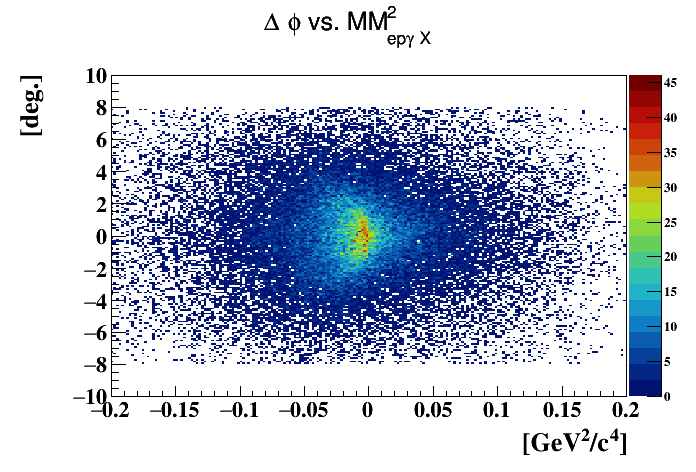
\includegraphics[height=5.6cm]{fig/delta_phi_epgamma_M2_Mis.png}
    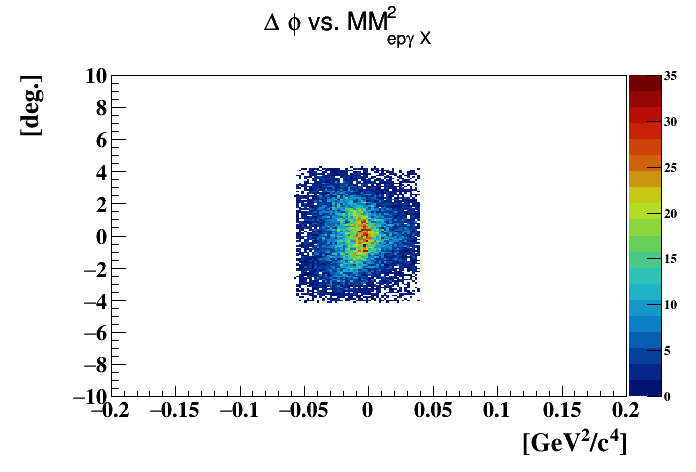
\includegraphics[height=5.6cm]{fig/delta_phi_epgamma_M2_Mis_with.png}
    \caption{ $\Delta \phi$ vs. $MM^{2}_{ep\gamma X}$ before (left) and 
    after (right) the exclusivity cuts.}
    \label{fig:2d_delta_phi_MM2_InCoh}
    \end{figure}                                                                  


  \item Produce all 9 plots in right figure of slides 5 and 9 of \url{ 
     https://clasweb.jlab.org/rungroups/lowq/wiki/images/a/a0/ExcluCuts-CANeg6.pdf}   
     for a 2$\sigma$ and 1$\sigma$ cuts on missing $ep\gamma X$ M2.\\
     \textcolor{blue}{The coherent and the incoherent distributions are 
        presented in figure \ref{fig:exc_Coh} and \ref{fig:exc_InCoh} 
     respectively. The reconstructed coherent and incoherent beam spin 
  asymmetries are presented in figures \ref{fig:exc_coh-alu} and 
  \ref{fig:exc_incoh-alu} respectively. In terms of the exclusivity 
  distributions, no correlations were observed in the coherent DVCS channel, 
  while a slight correlation was observed between the $ep\gamma$ MM2 and $epX$ 
  MM2.} \textcolor{red}{Do we have to apply tighter cuts in the incoherent 
  case?.}

  \begin{figure}[tbp]
    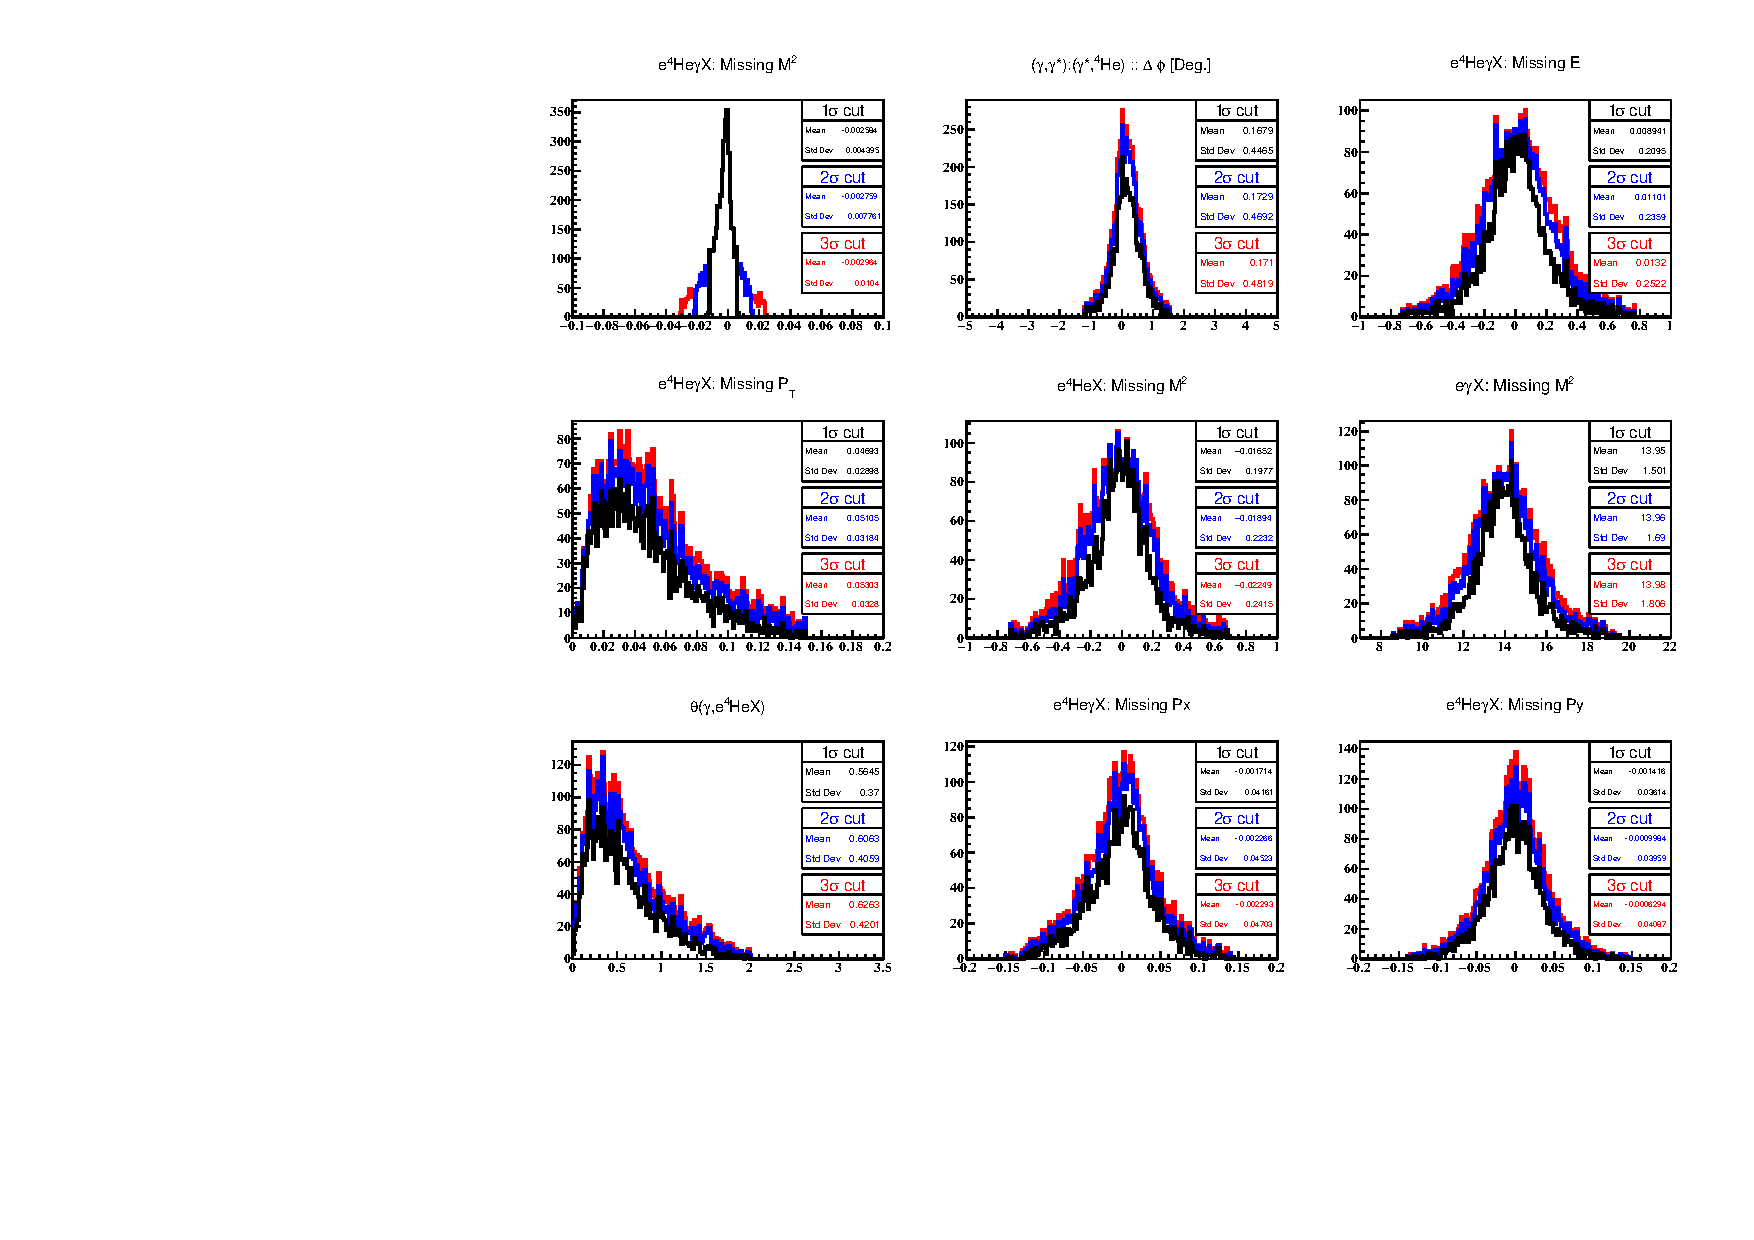
\includegraphics[height=14.6cm]{fig/all_sigmas_coh_exc_cuts.pdf}
    \caption{Coherent exclusivity distributions corresponding to different cuts 
    on $e^{4}He\gamma X$ missing mass squared.}
    \label{fig:exc_Coh}
    \end{figure}

    \begin{figure}[tbp]
    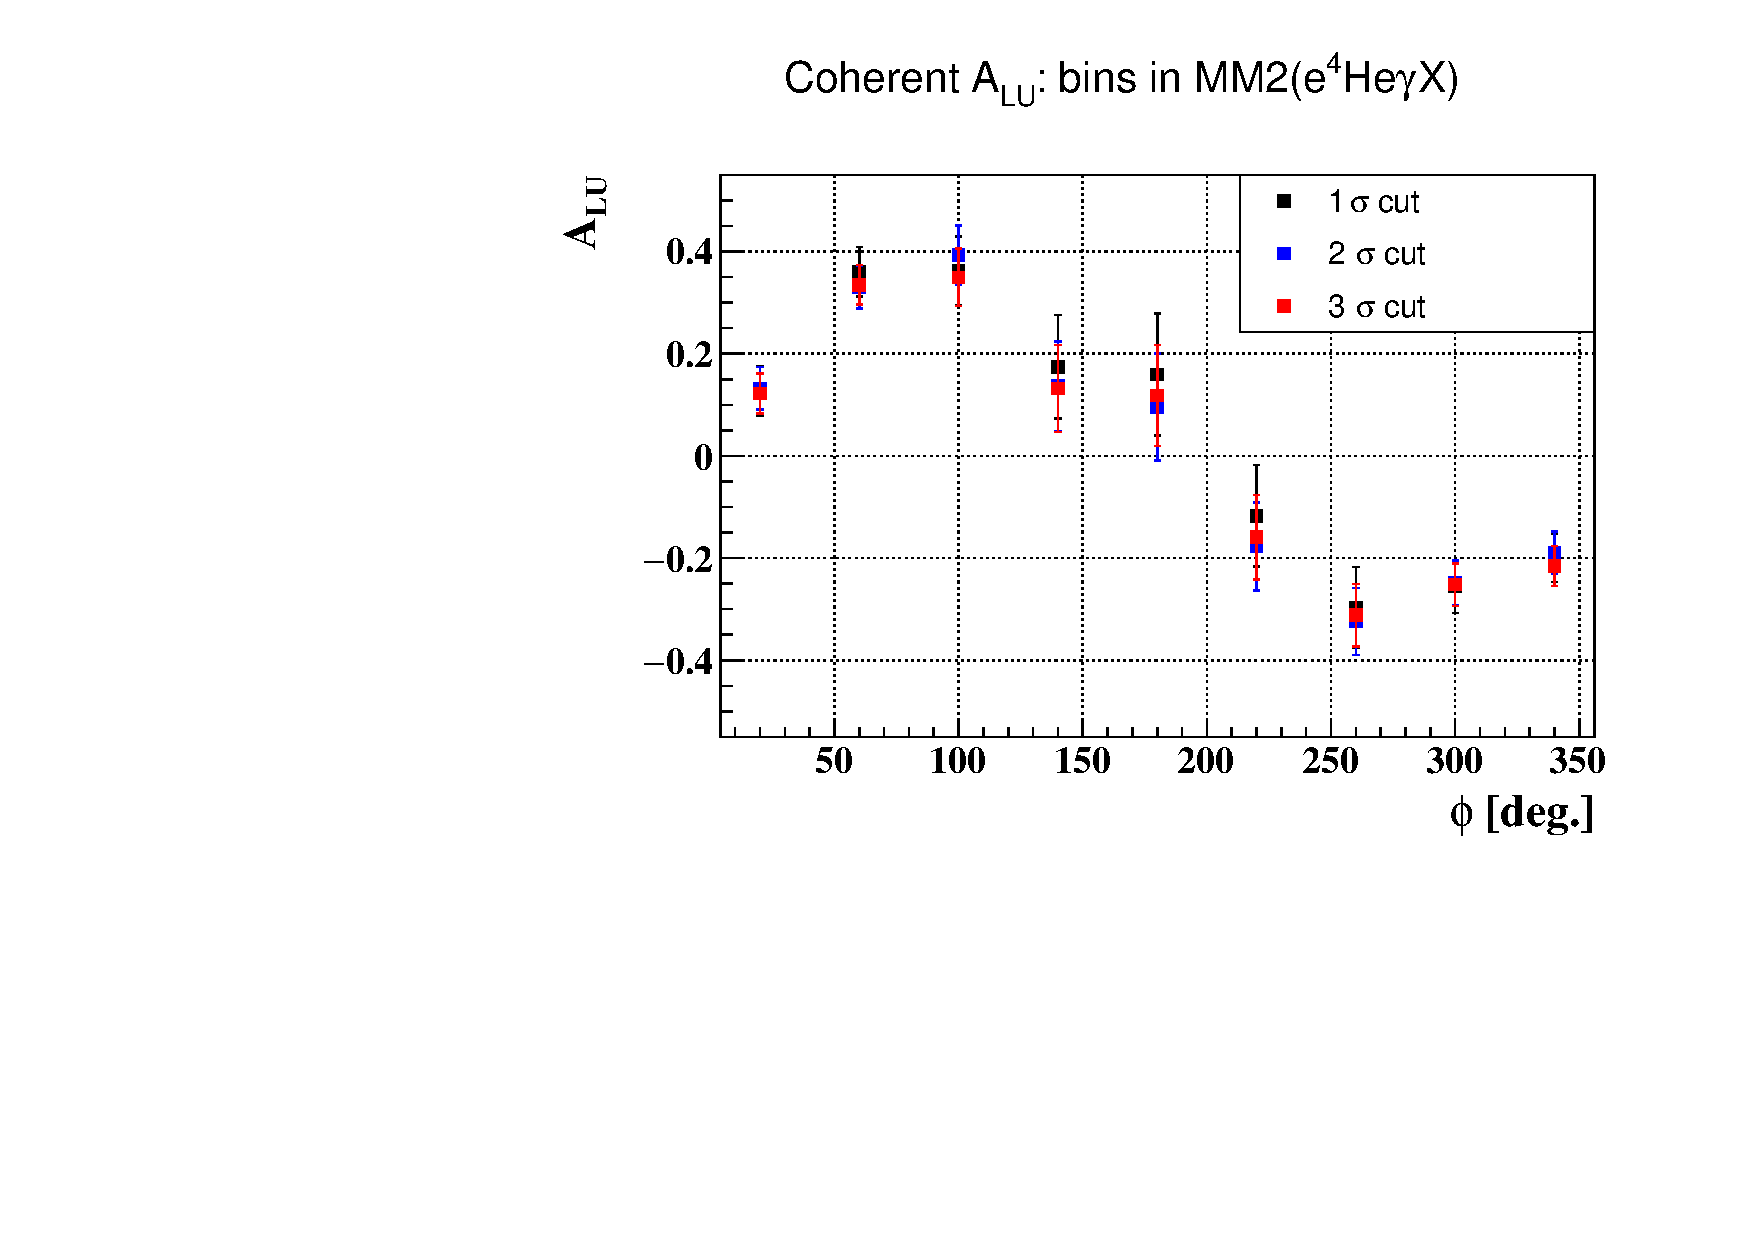
\includegraphics[height=6.0cm]{fig/ALU_coherent_MM2.pdf}
    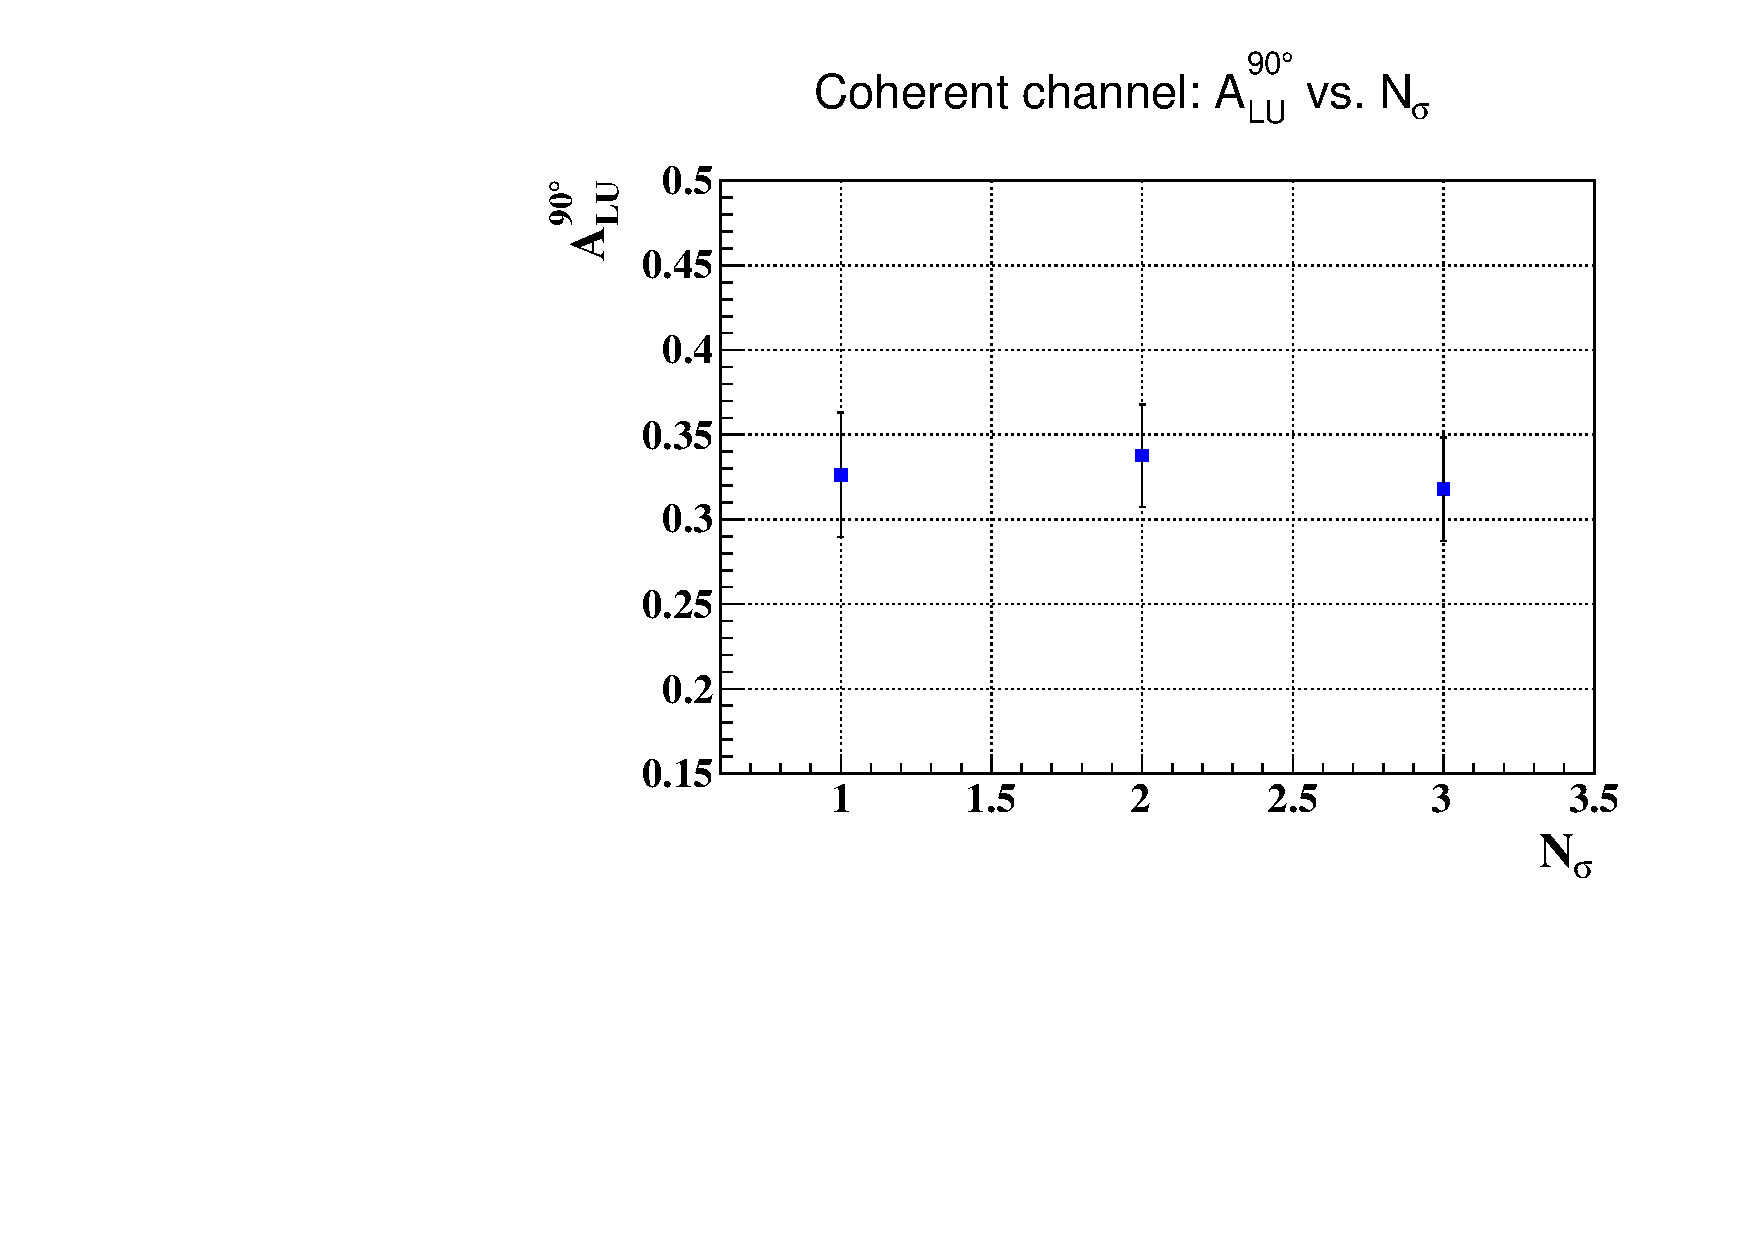
\includegraphics[height=6.0cm]{fig/ALU_coherent_MM2_90deg.pdf}
    \caption{On the left: the integrated coherent beam-spin asymmetries as a 
    function of $\phi$ corresponding to different cuts on $e^{4}He\gamma X$ 
 missing mass squared. On the right: $A_{LU}$ at 90$^{\circ}$ from fitting the
  reconstructed asymmetries as a function of the cut width.}
    \label{fig:exc_coh-alu}
    \end{figure} 

    \begin{figure}[tbp]
    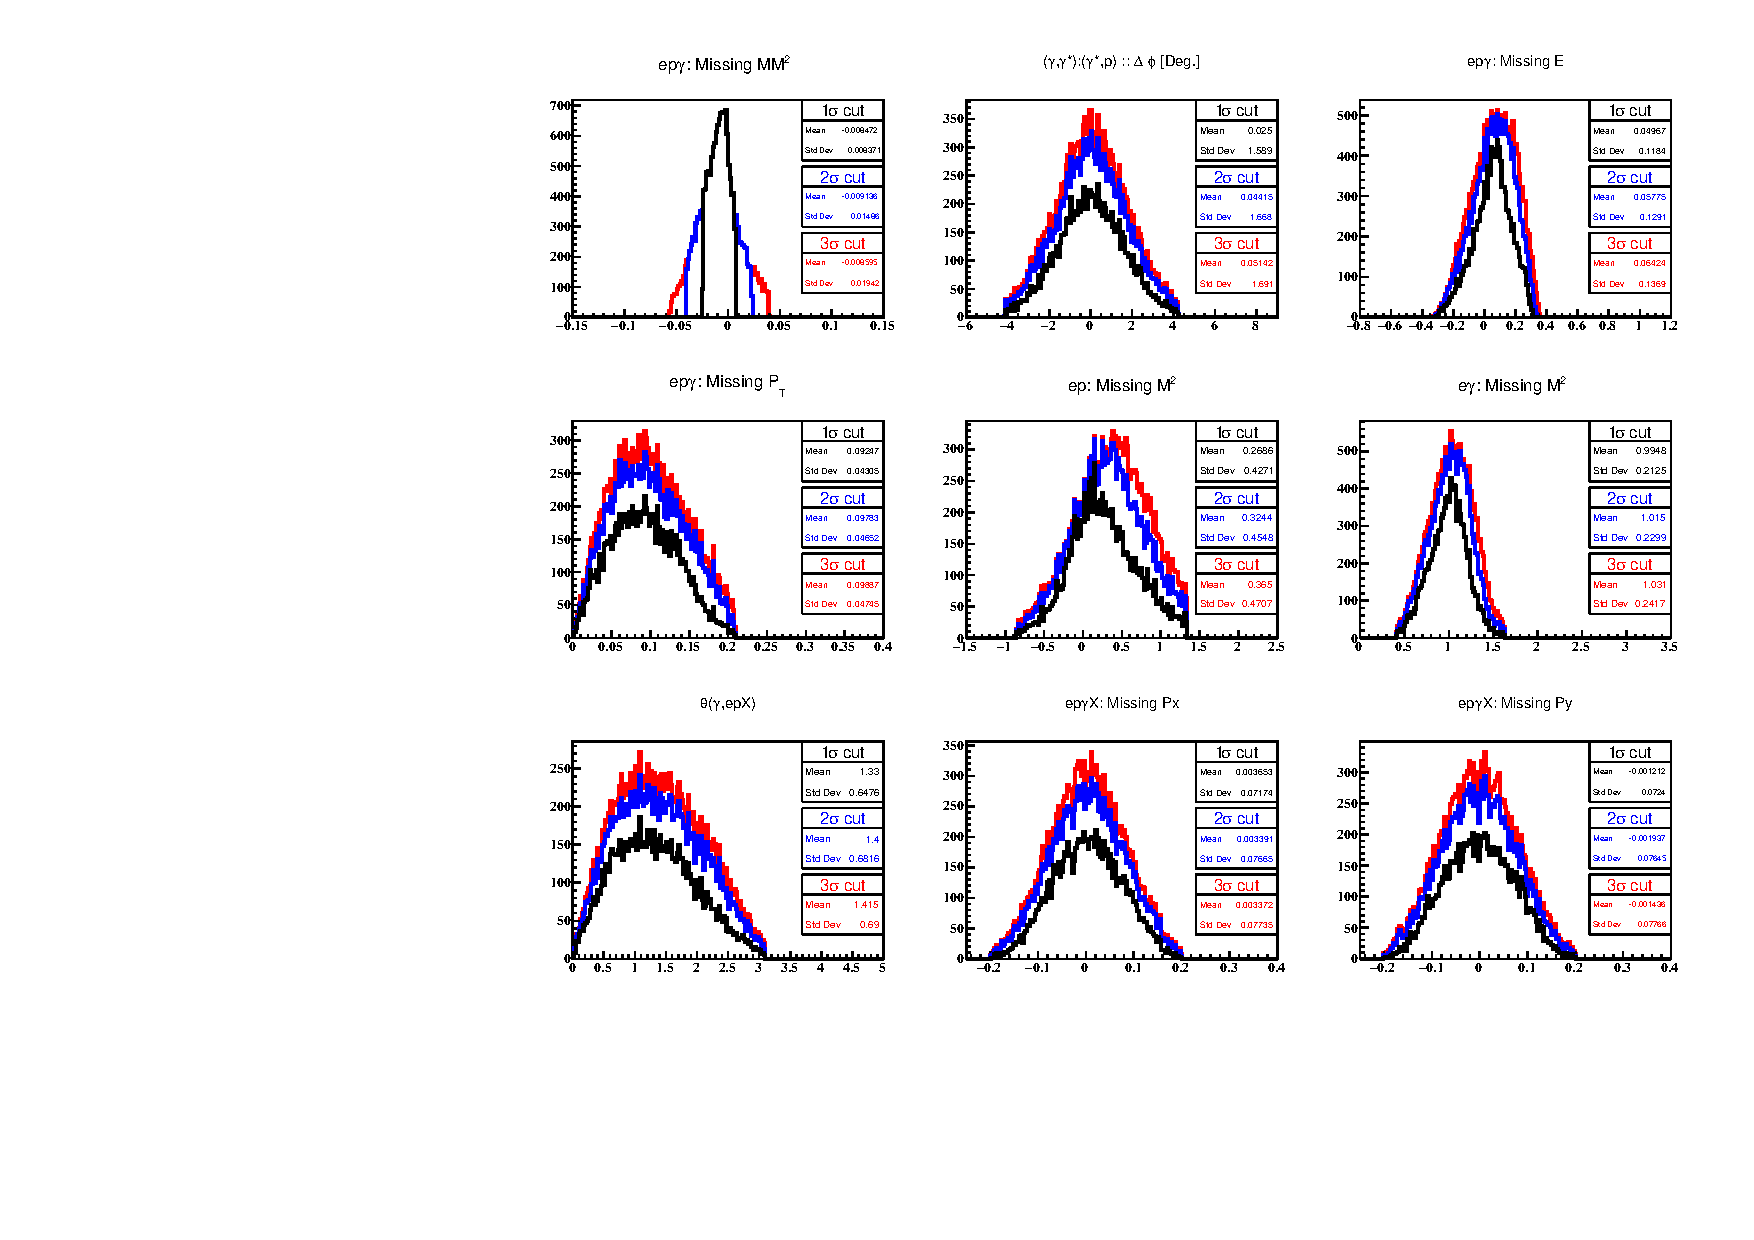
\includegraphics[height=14.6cm]{fig/all_sigmas_incoh_exc_cuts.pdf}
    \caption{ Incoherent exclusivity distributions for the different cuts on 
    $ep\gamma X$ missing mass squared.}
    \label{fig:exc_InCoh}
    \end{figure}                                                                  


    \begin{figure}[tbp]
    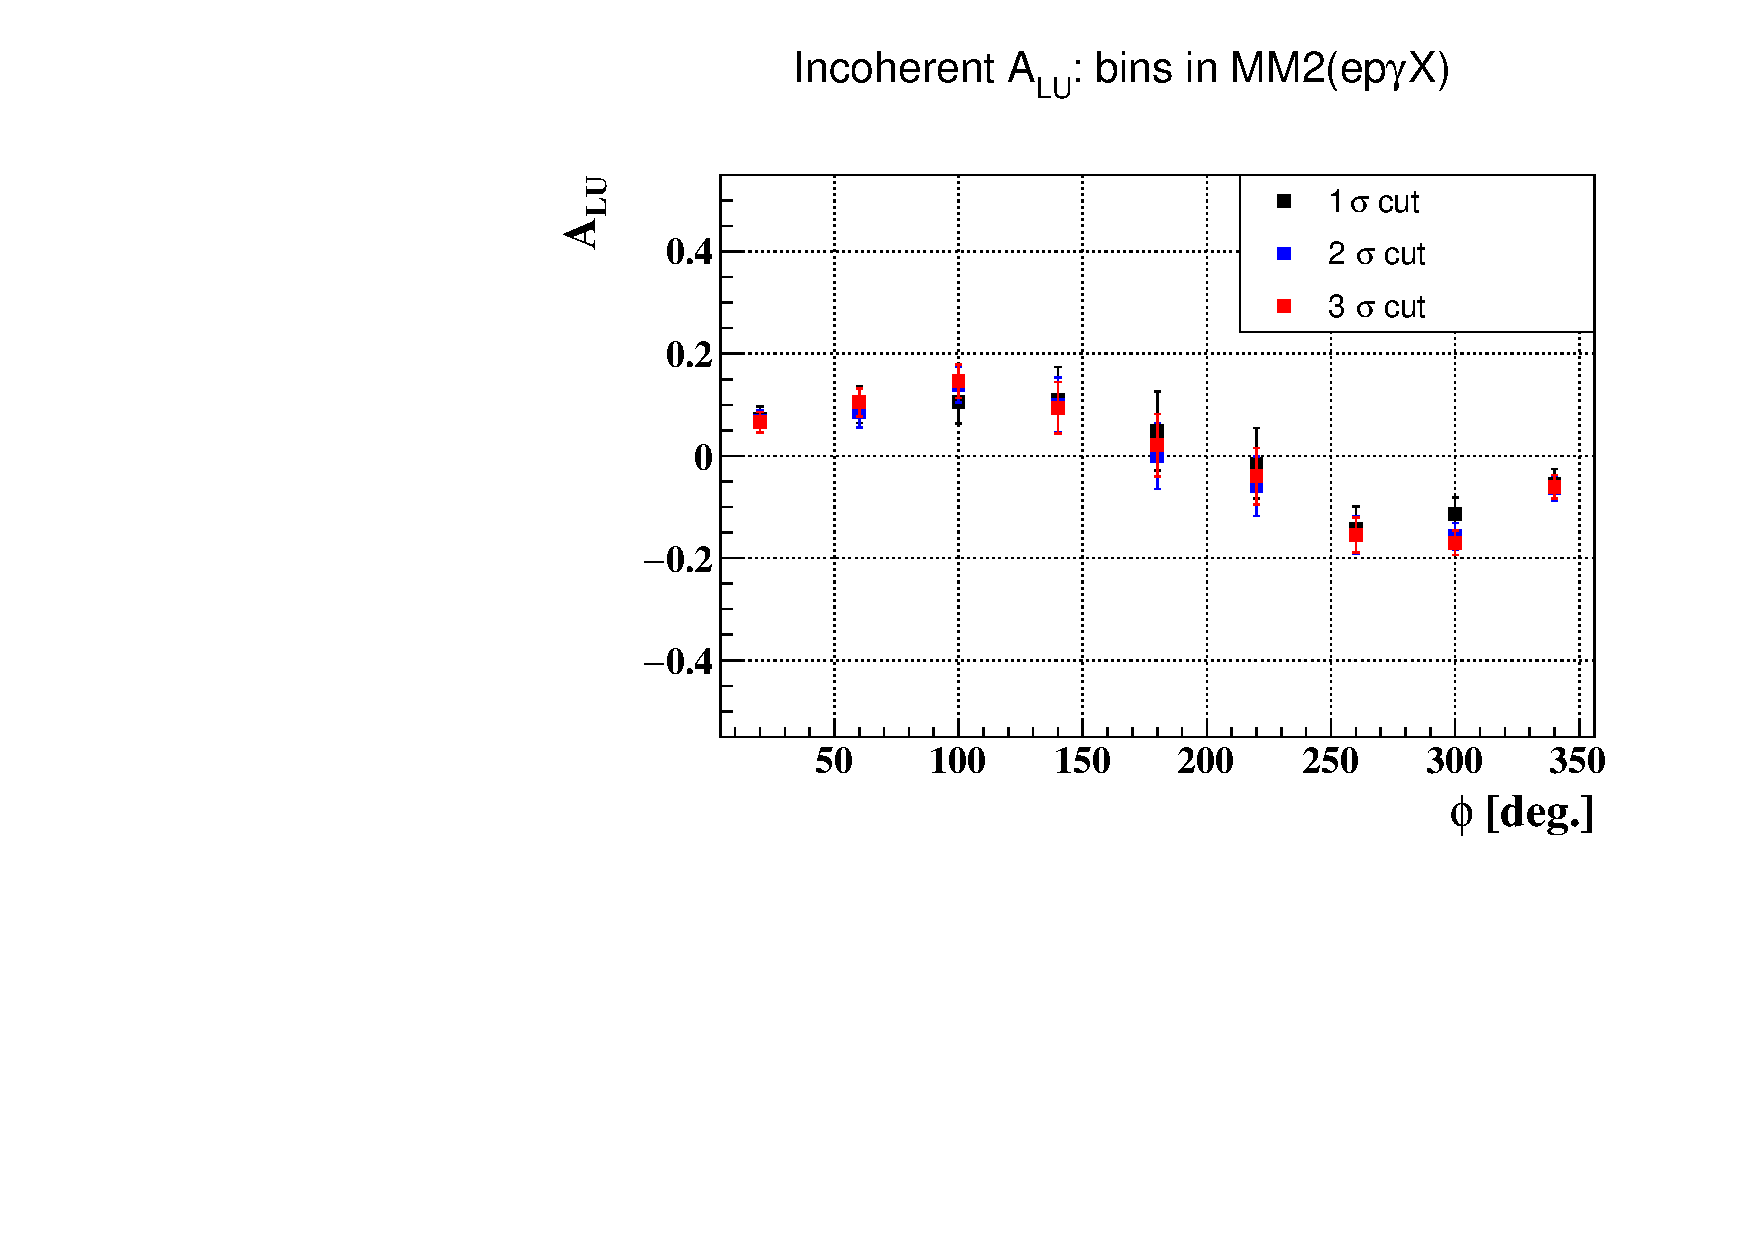
\includegraphics[height=6.0cm]{fig/ALU_incoherent_MM2.pdf}
    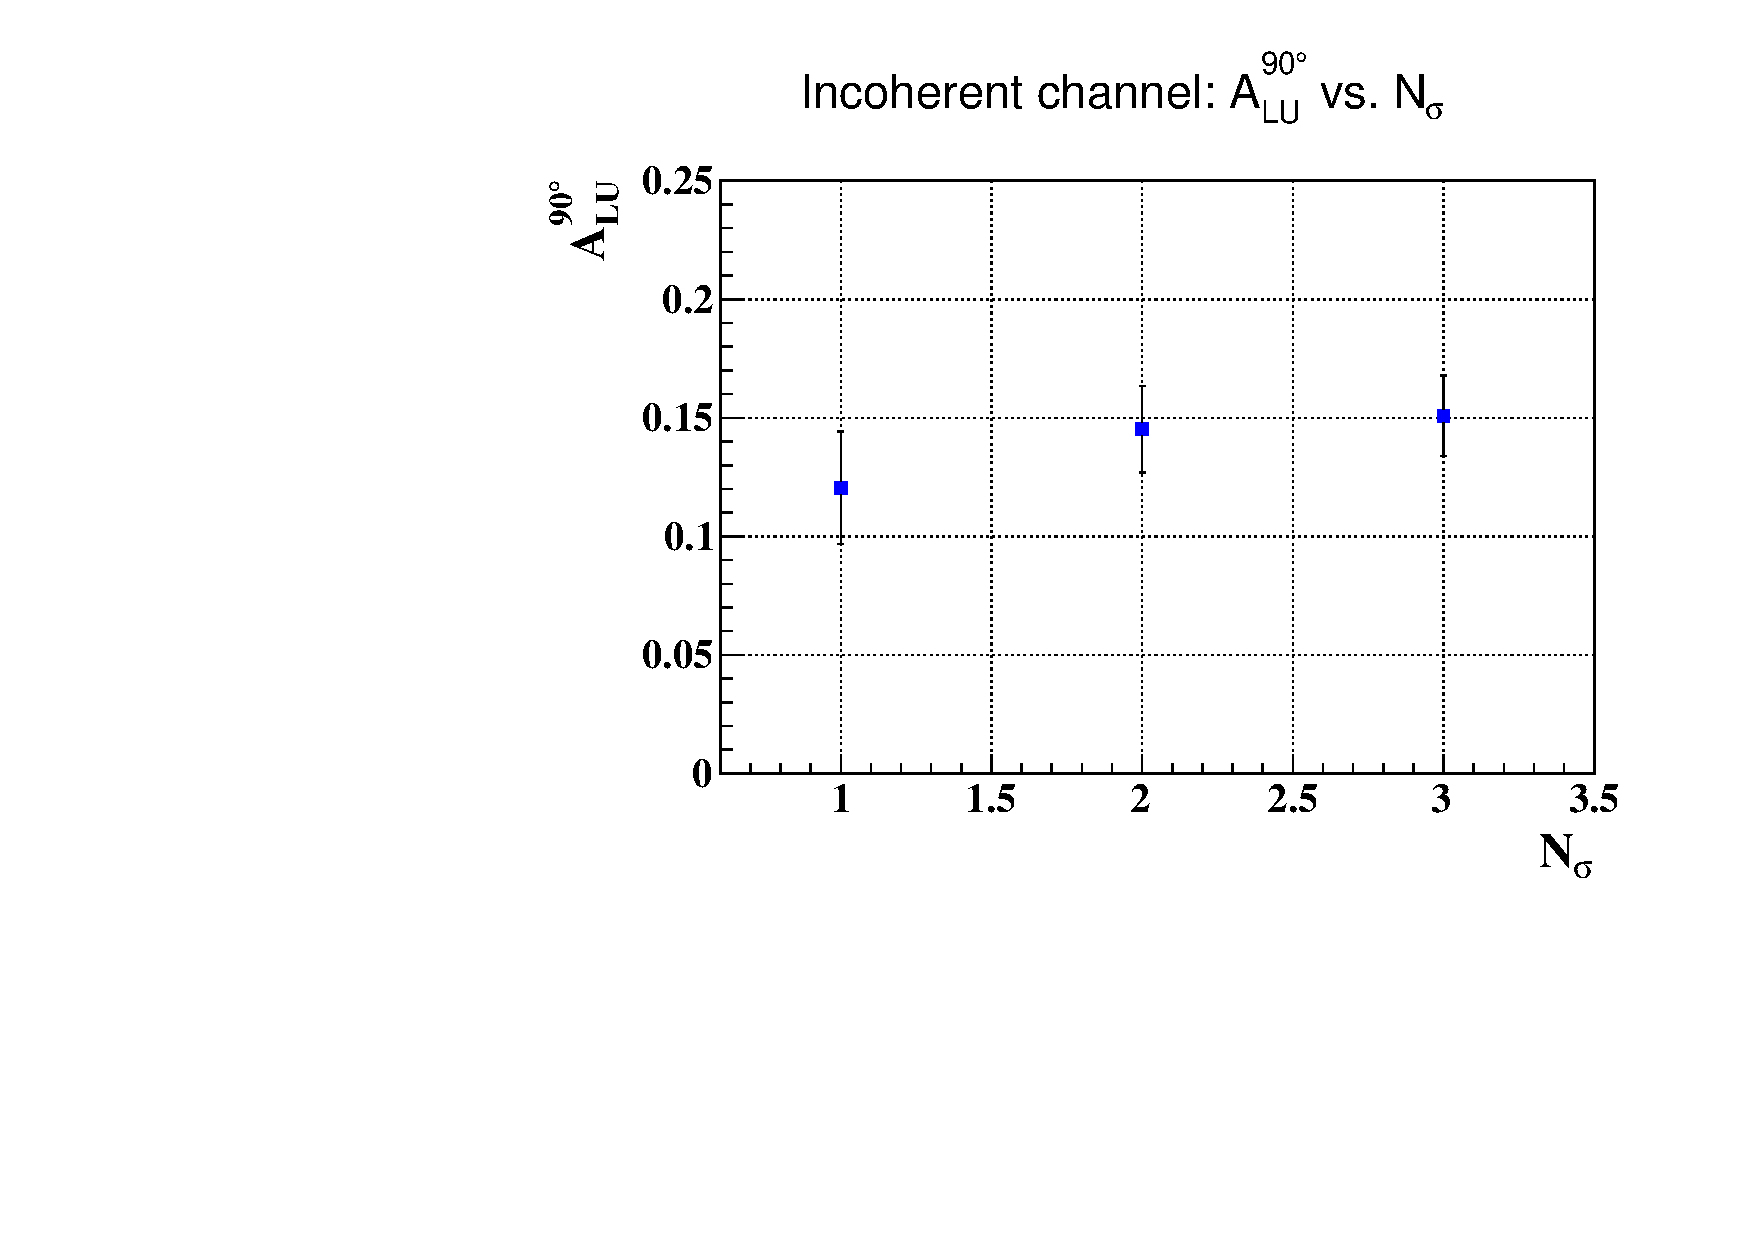
\includegraphics[height=6.0cm]{fig/ALU_incoherent_MM2_90deg.pdf}
    \caption{On the left: the integrated incoherent beam-spin asymmetries as a 
    function of $\phi$ corresponding to different cuts on $e^{4}He\gamma X$ 
 missing mass squared. On the right: $A_{LU}$ at 90$^{\circ}$ from fitting the 
 reconstructed asymmetries as a function of the cut width.}
    \label{fig:exc_incoh-alu}
    \end{figure} 




    \end{enumerate}
\item (optionally) In the incoherent case, extract ALU with 2 variations of the 
   ep missing M2 right cut, moving it tighter to the left (e.g. 1 and 0.75 
   GeV2).  (also see the evolution of the other distributions when doing so).\\
   \textcolor{blue}{The reconstructed incoherent asymmetries are presented in 
      figure \ref{fig:BSA_incoherent_epMM} with the associated exlcusive 
      distributions in figure \ref{fig:epMM2_incoh_exc_cuts}. The different 
   tail cuts show no major effects on the reconstructed ALU.}

   \begin{figure}[tbp]
    \centering
    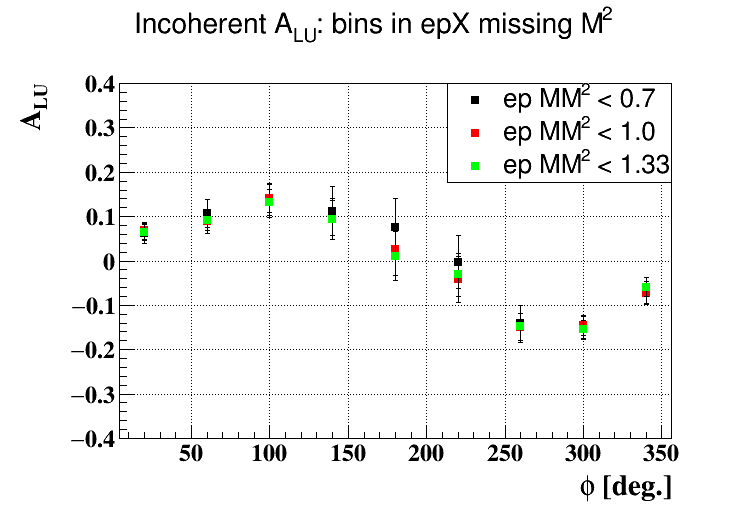
\includegraphics[height=8.6cm]{fig/BSA_incoherent_epMM.png}
    \caption{ The integrated, over $Q^{2}$, $x_{B}$, and $-t$, incoherent 
    beam-spin asymmetries as a function of $\phi$ for the different cuts on 
 $epX$ missing mass squared.}
    \label{fig:BSA_incoherent_epMM}
    \end{figure}                                                                

    \begin{figure}[tbp]
    \centering
    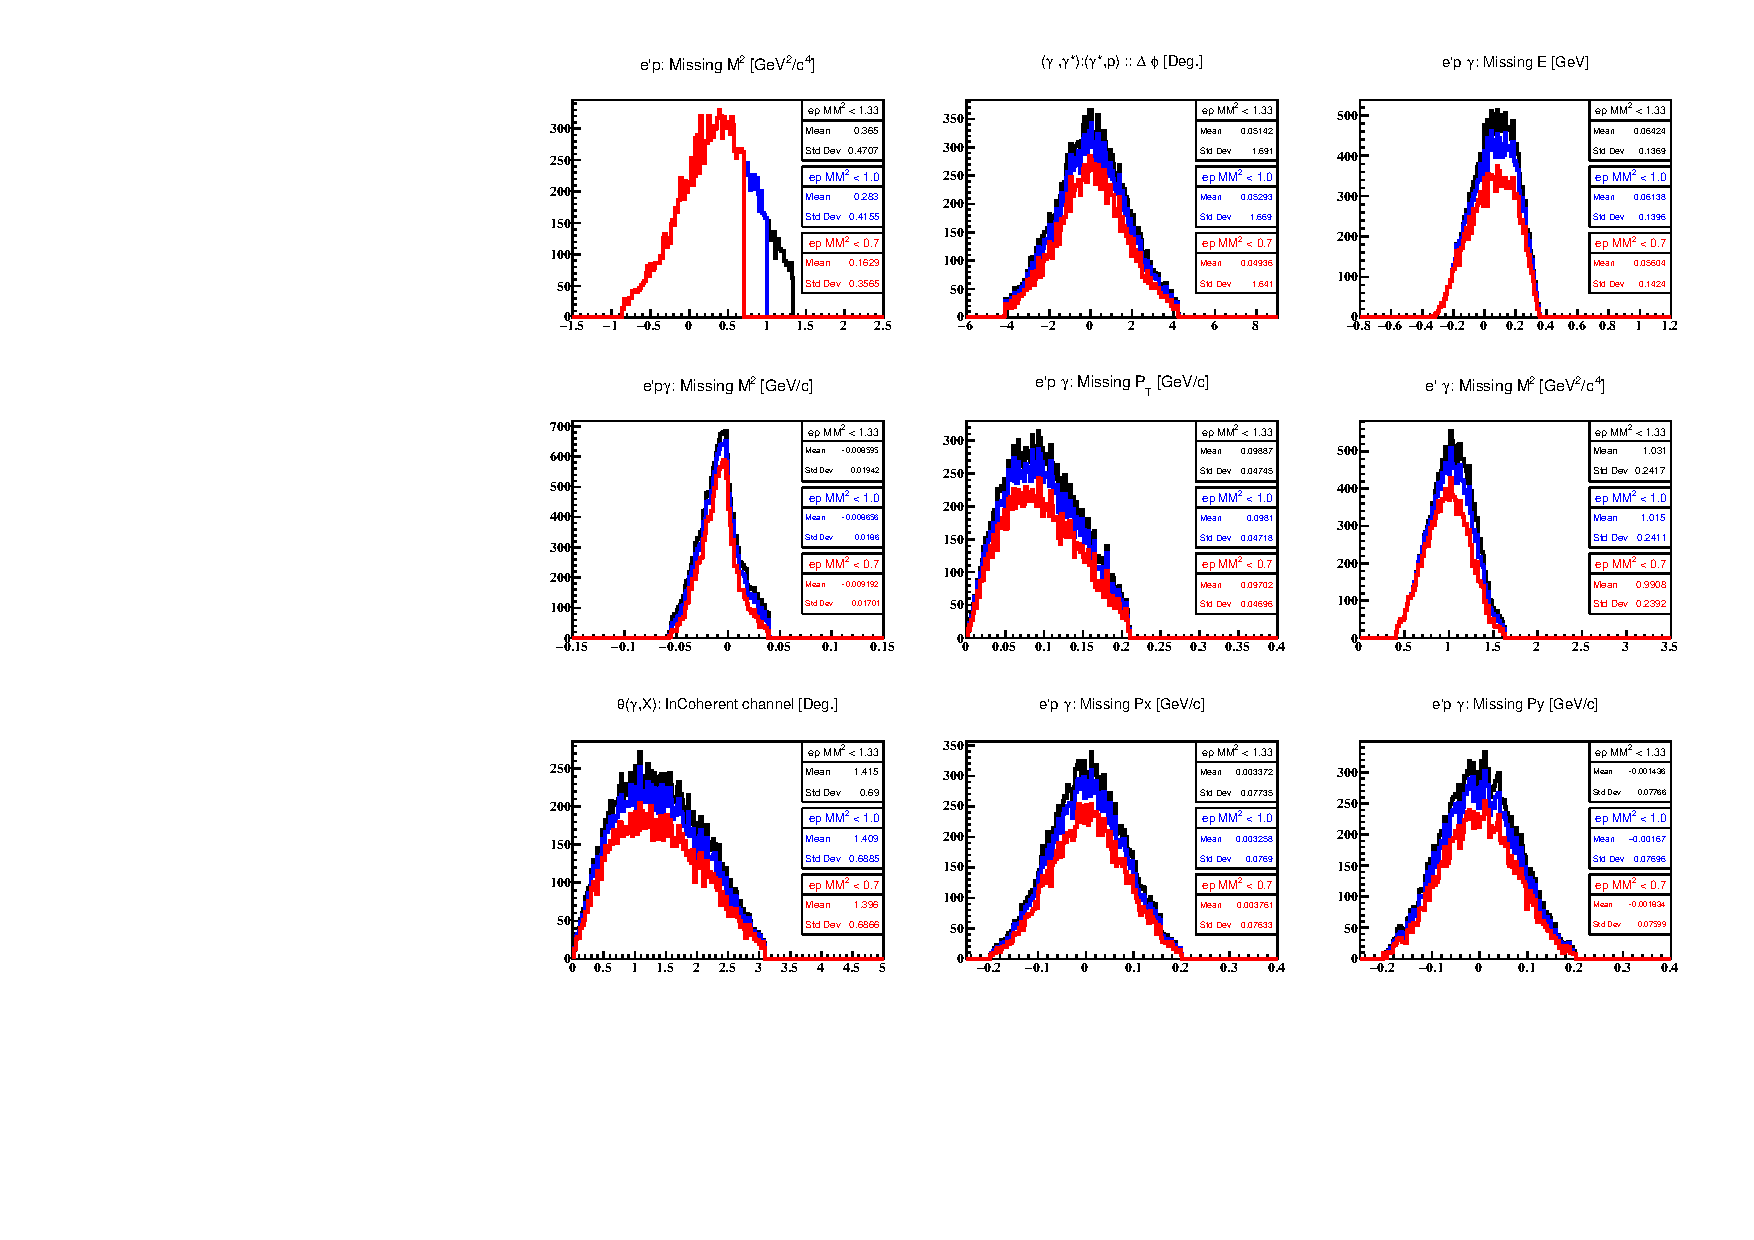
\includegraphics[height=14.6cm]{fig/epMM2_incoh_exc_cuts.pdf}
    \caption{ Incoherent exclusivity distributions for the different cuts on 
    $epX$ missing mass squared.}
    \label{fig:epMM2_incoh_exc_cuts}
    \end{figure}                                                                  


\end{enumerate}

\item Free proton asymmetries from FX's publication: implement a (possibly 3D/9 
points) interpolation to smooth out both statistical fluctuations and 
kinematical dependences. Reintroduce a corresponding section in the CAN. Take 
into account both stat. and syst. errors of both experiments in the ratio. The 
committee recommends though to be cautious about the statements on the 
asymmetry ratios in the future publication.
  \begin{figure}[tbp]
    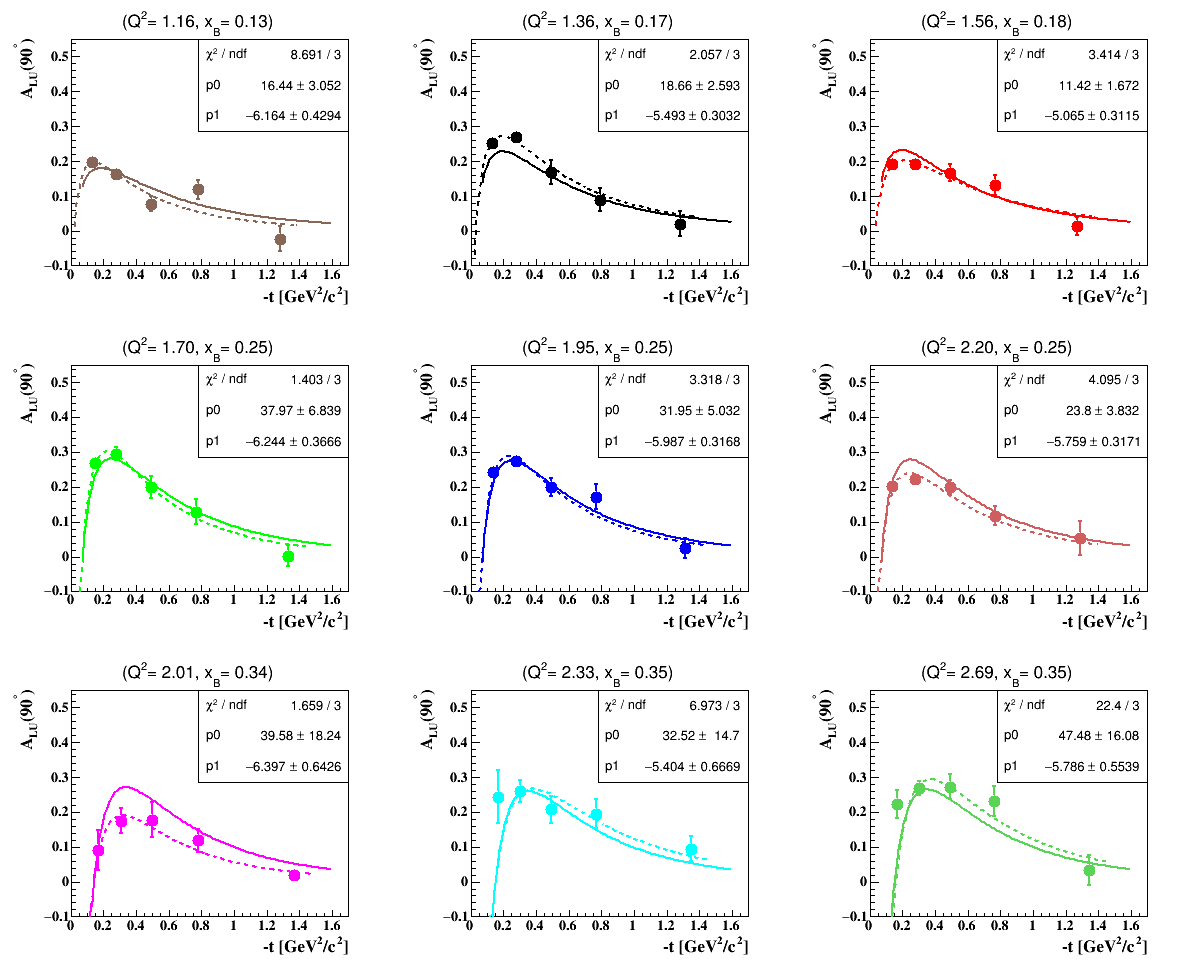
\includegraphics[height=14.6cm]{fig/ALU-proton-fits.png}
    \caption{ Fitting e1dvcs1 free proton beam-spin asymmetries. The dashed 
    curves are fits to the data in the form of 
 $p_{0}*(t-t_{min})*e^{p_{1}*\sqrt{t}}$, while the solid curves are from 
 calculations based on fitting the parameters $p_{0}$ and $p_{1}$.}
    \label{fig:free-proton-alu-fits}
    \end{figure}

  \begin{figure}[tbp]
    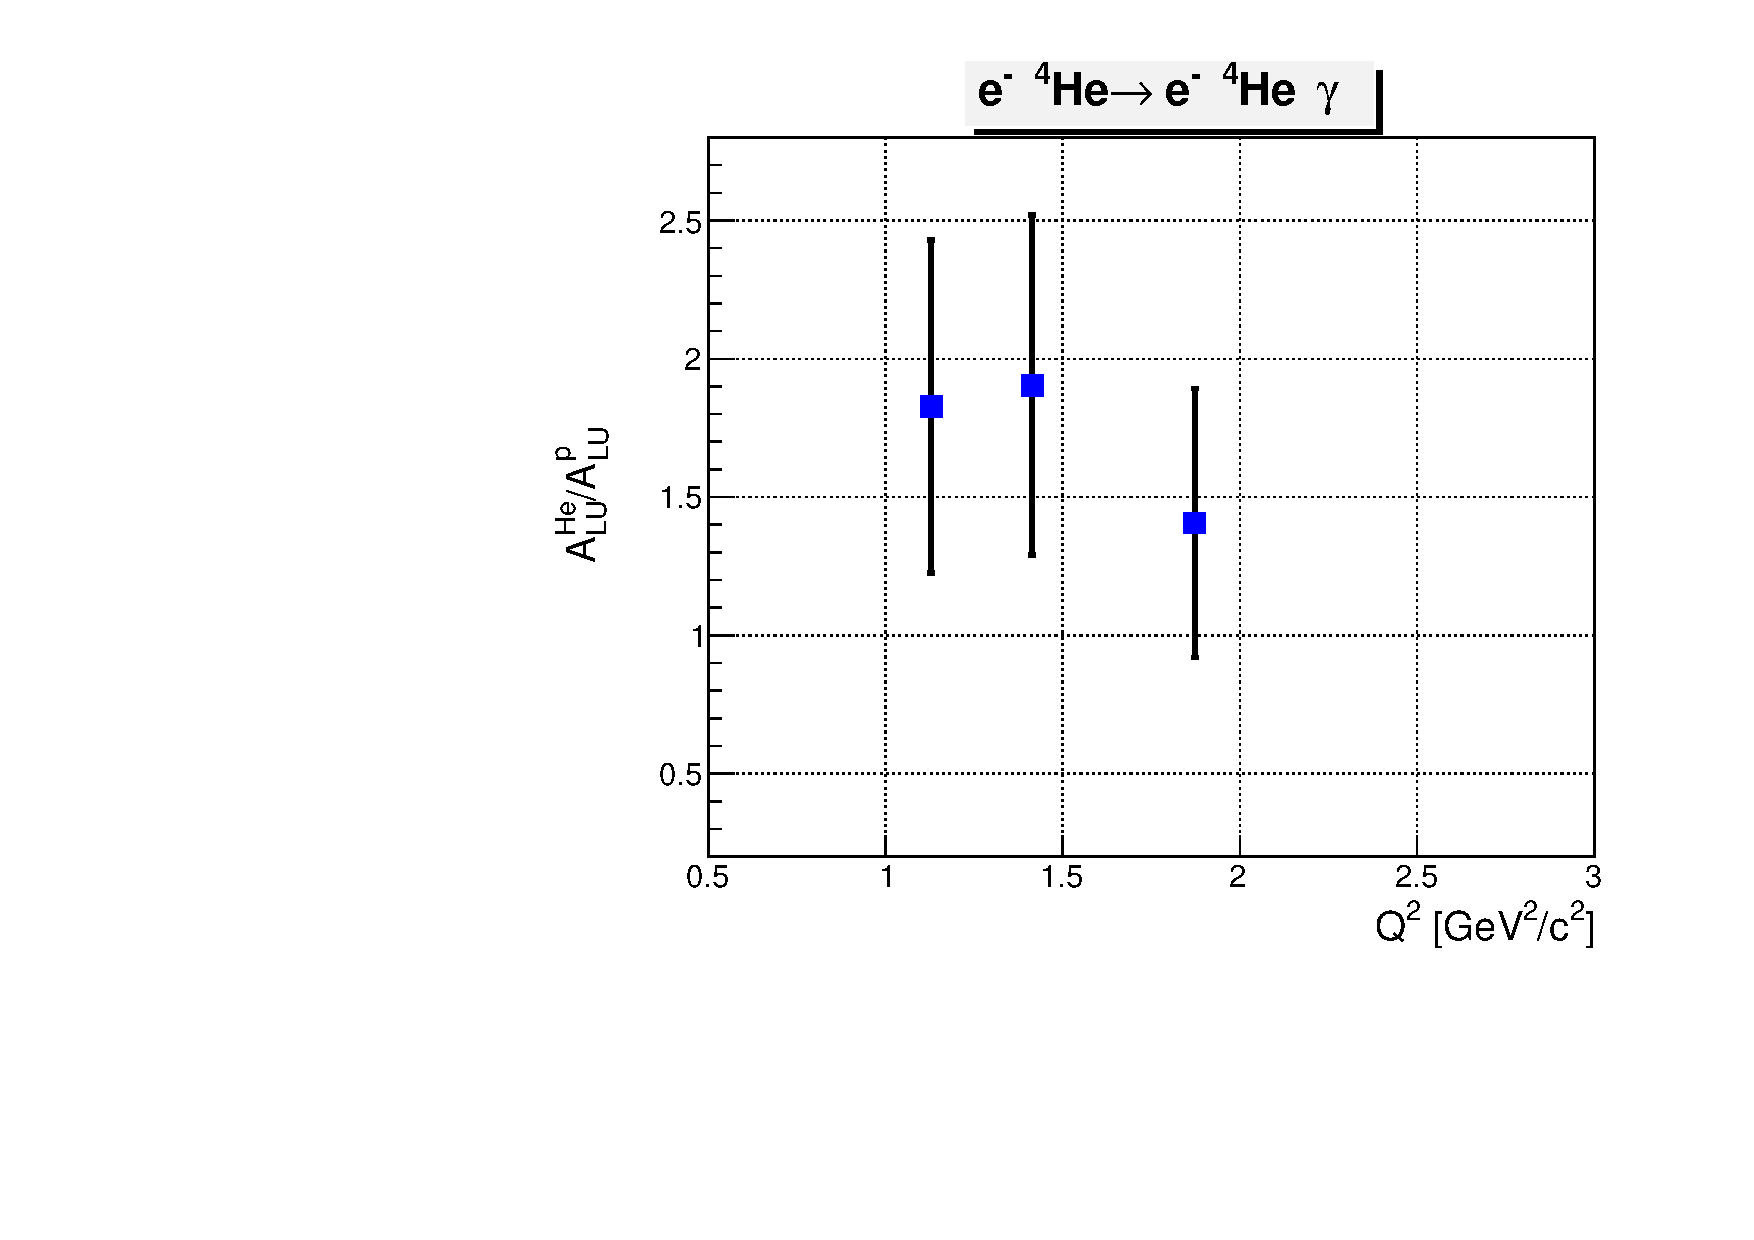
\includegraphics[height=6.6cm]{fig/BSA_ratio_coh_Q2.pdf}
    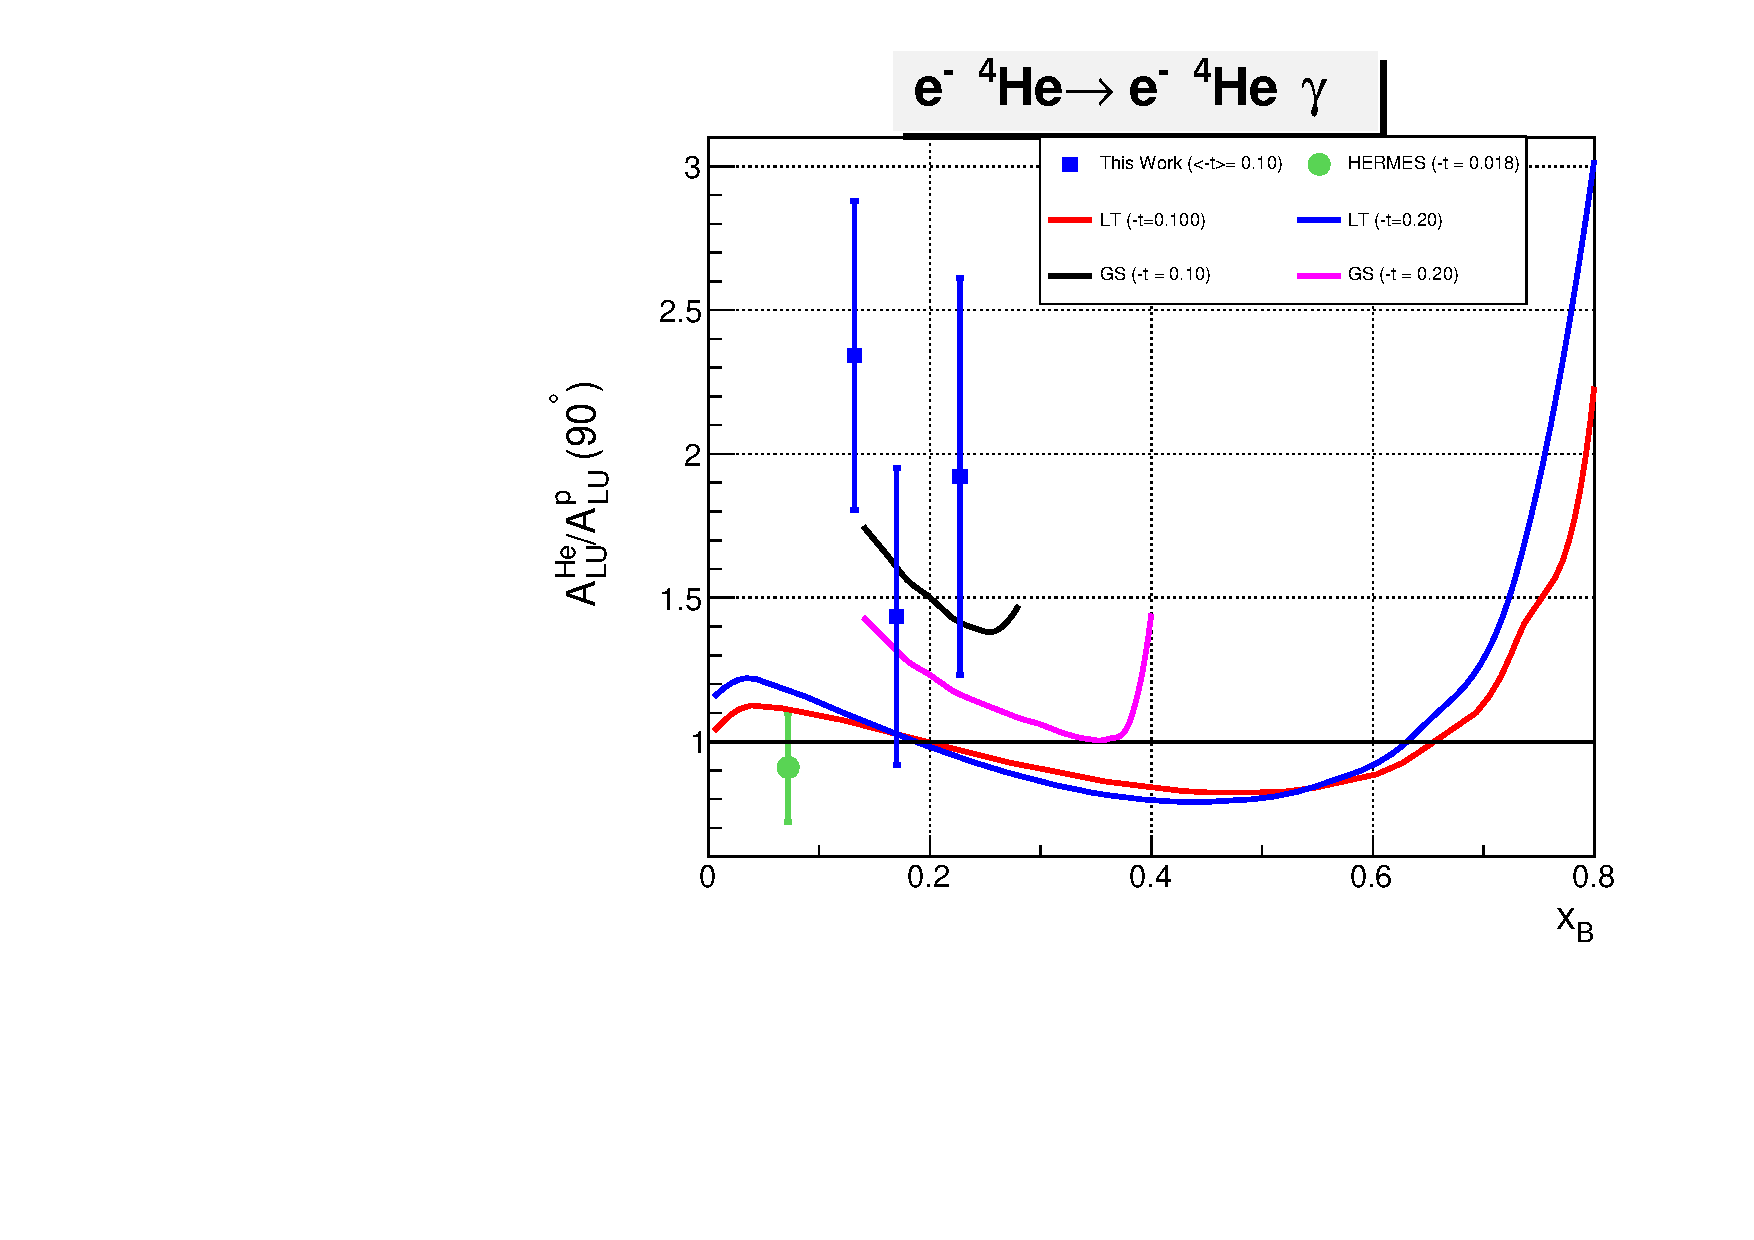
\includegraphics[height=6.6cm]{fig/BSA_ratio_coh_x.pdf}
    \centering
    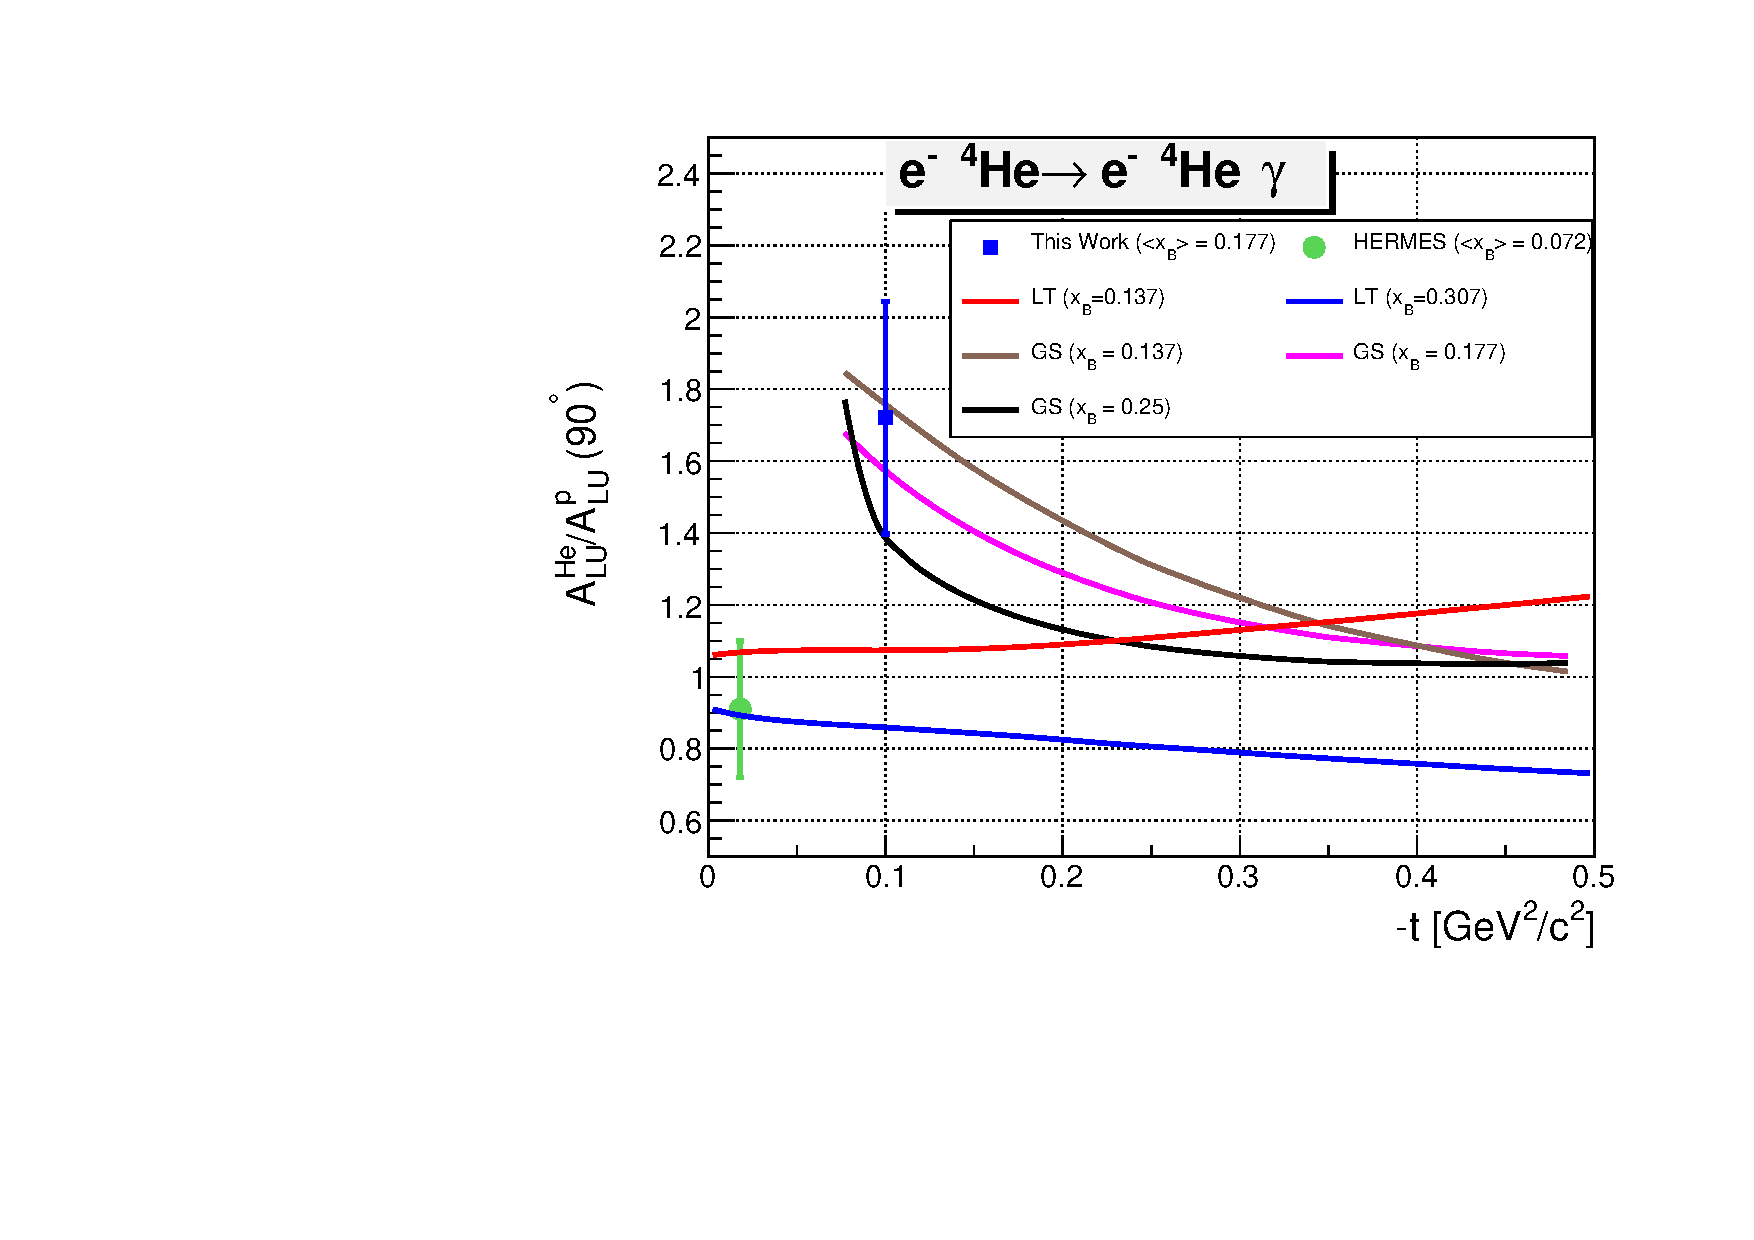
\includegraphics[height=6.6cm]{fig/BSA_ratio_coh_t.pdf}
    \caption{ $A_{LU}$ ratio between $^{4}$He DVCS and free proton at $\phi = 
    90 ^{\circ}$ as a function of $Q^{2}$, $x_{B}$, and $-t$.}
    \label{fig:coh-alu-ratios}
    \end{figure}

 \begin{figure}[tbp]
    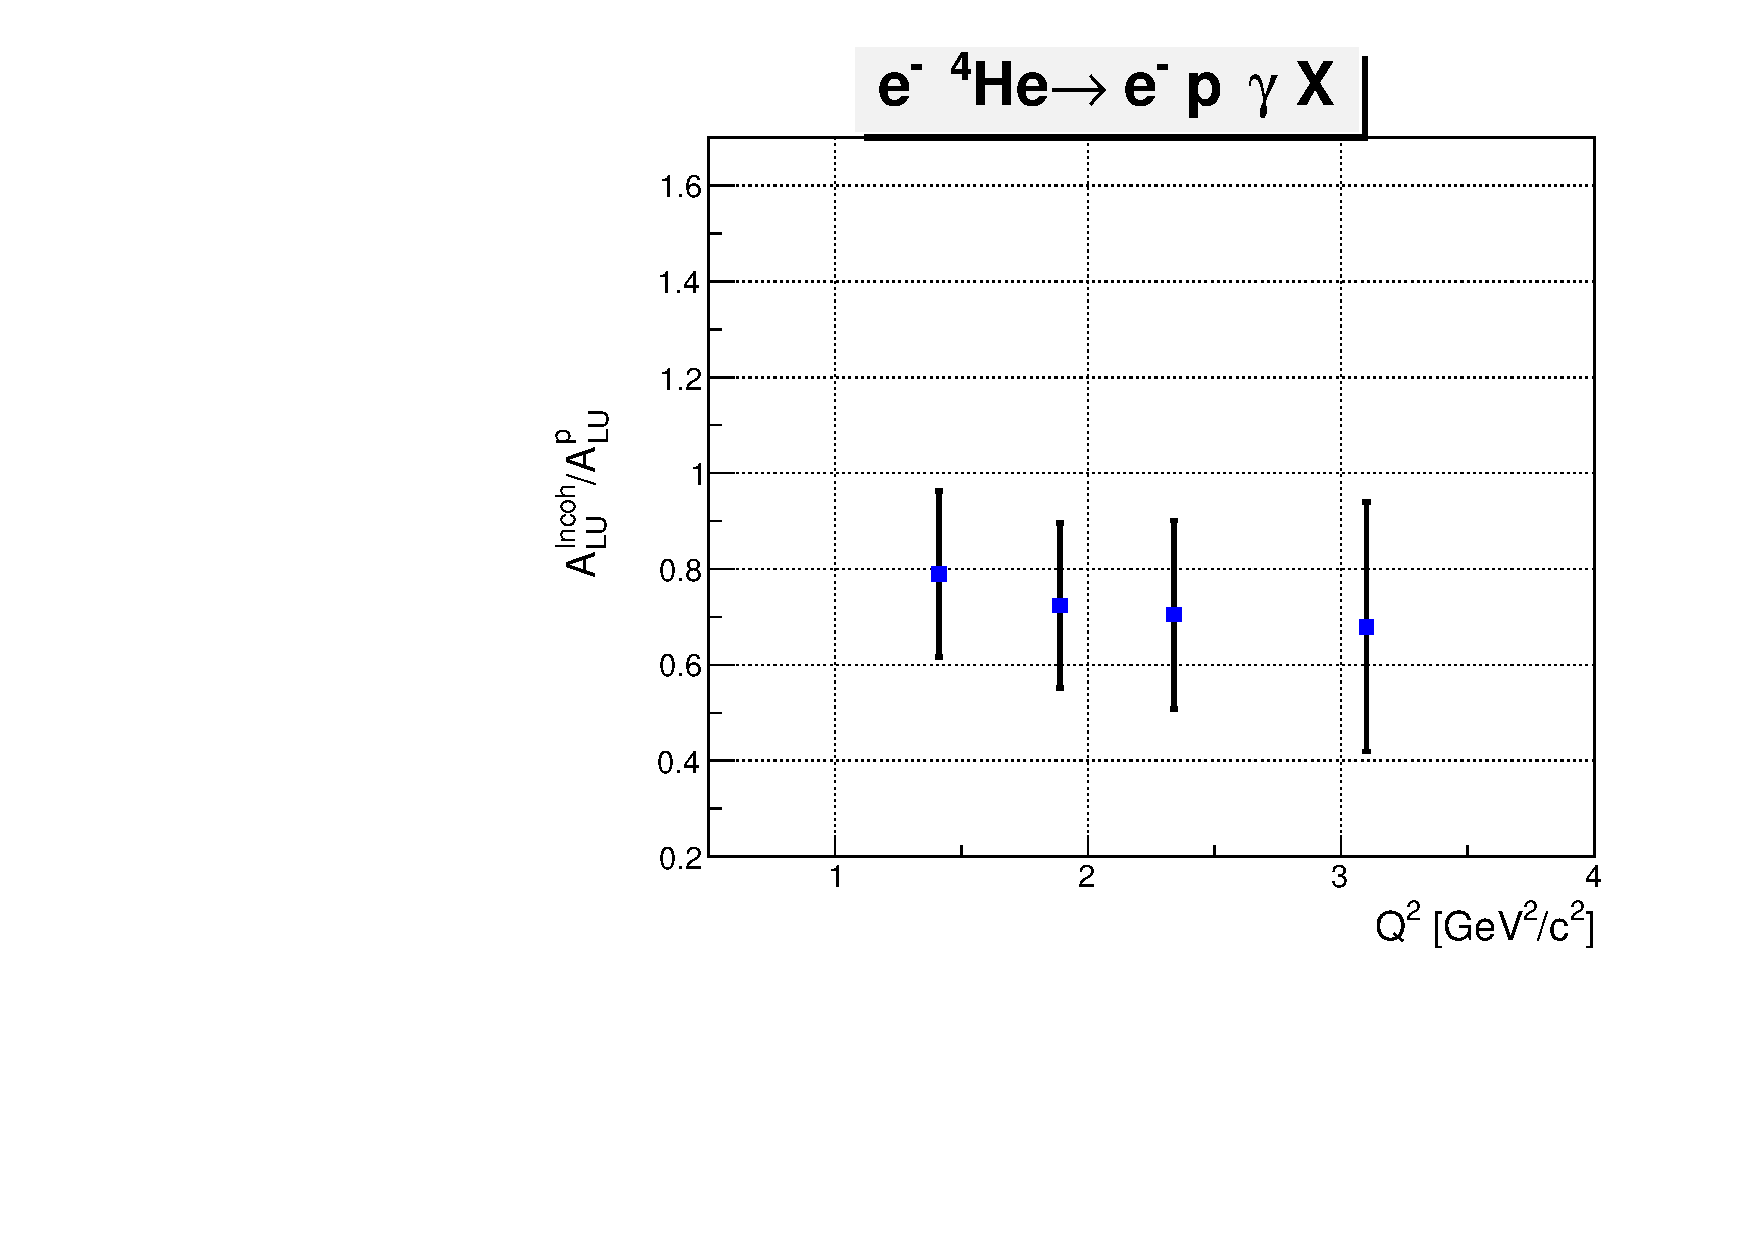
\includegraphics[height=6.6cm]{fig/BSA_ratio_incoh_Q2.pdf}
    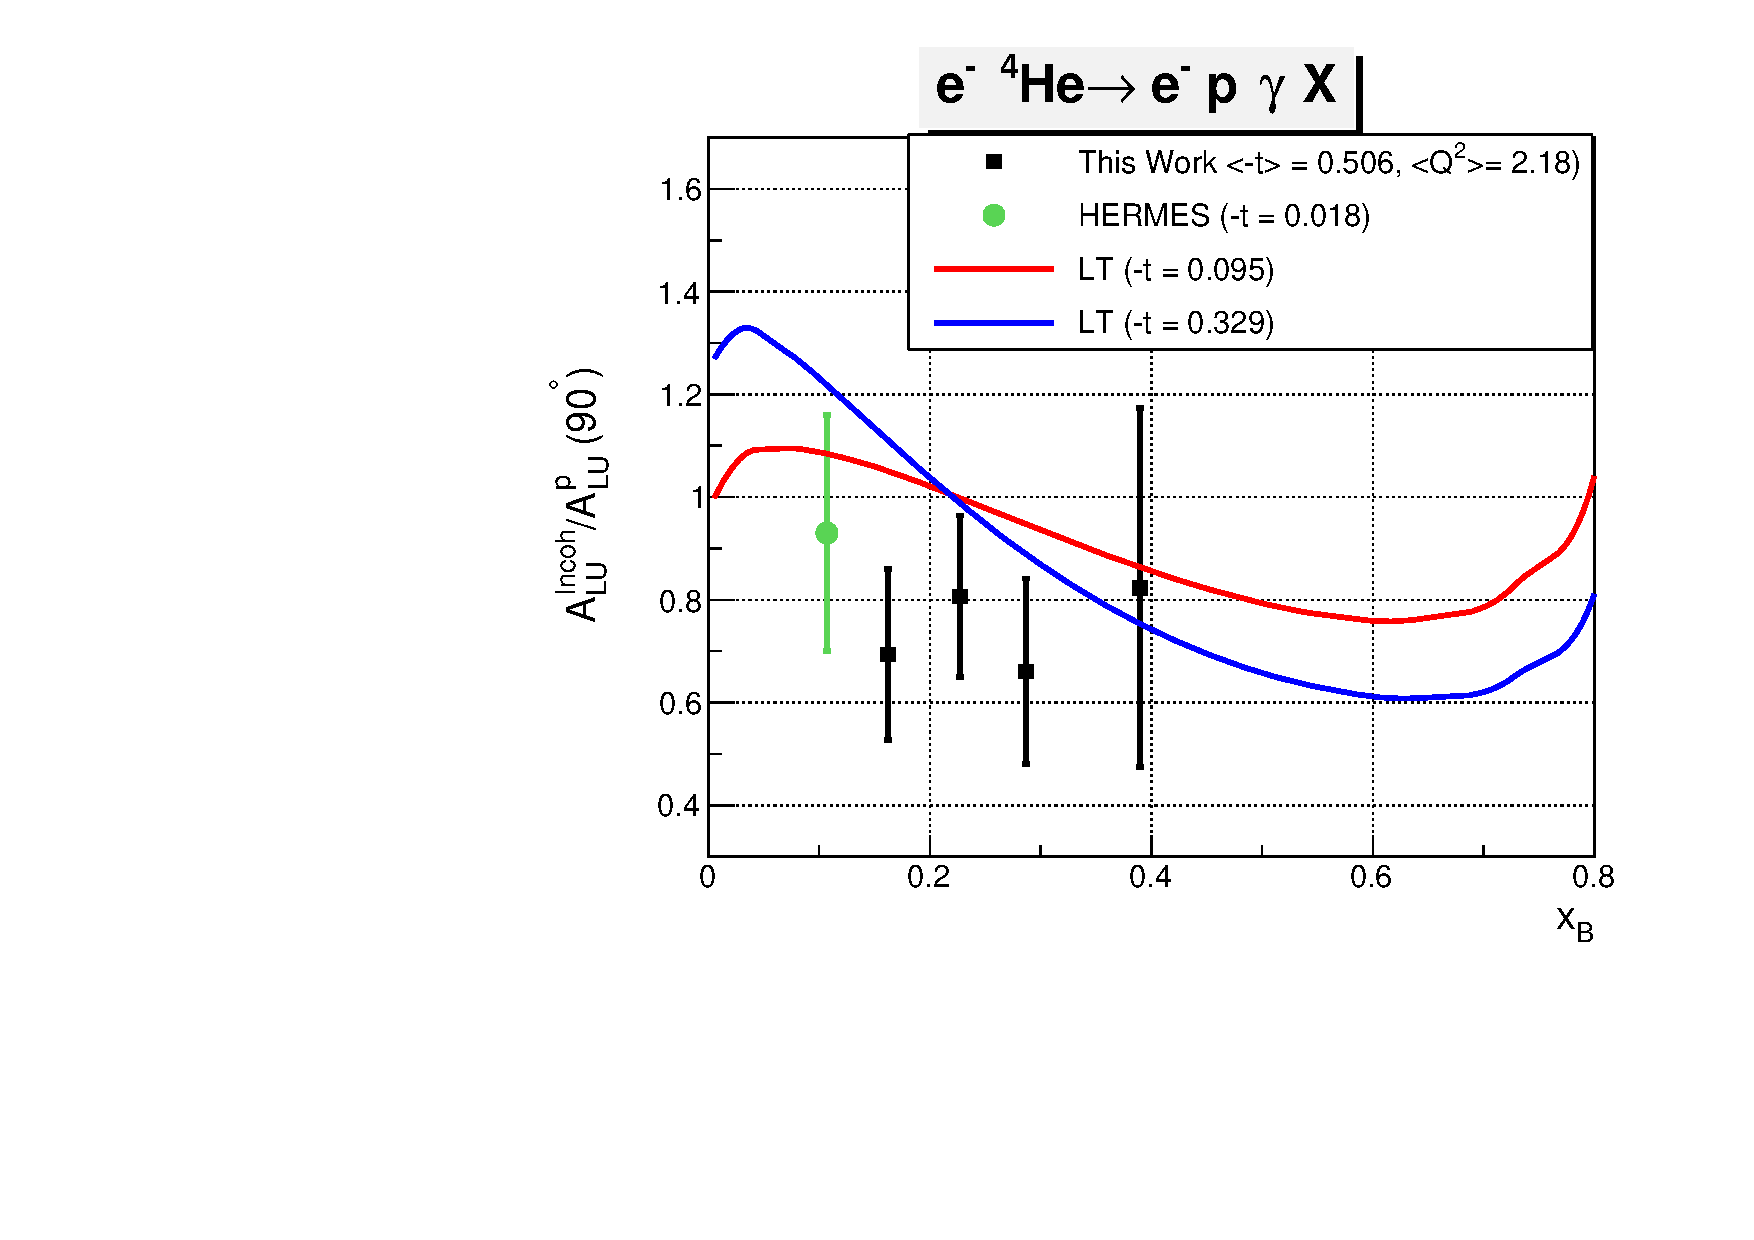
\includegraphics[height=6.6cm]{fig/BSA_ratio_incoh_x.pdf}
    \centering
    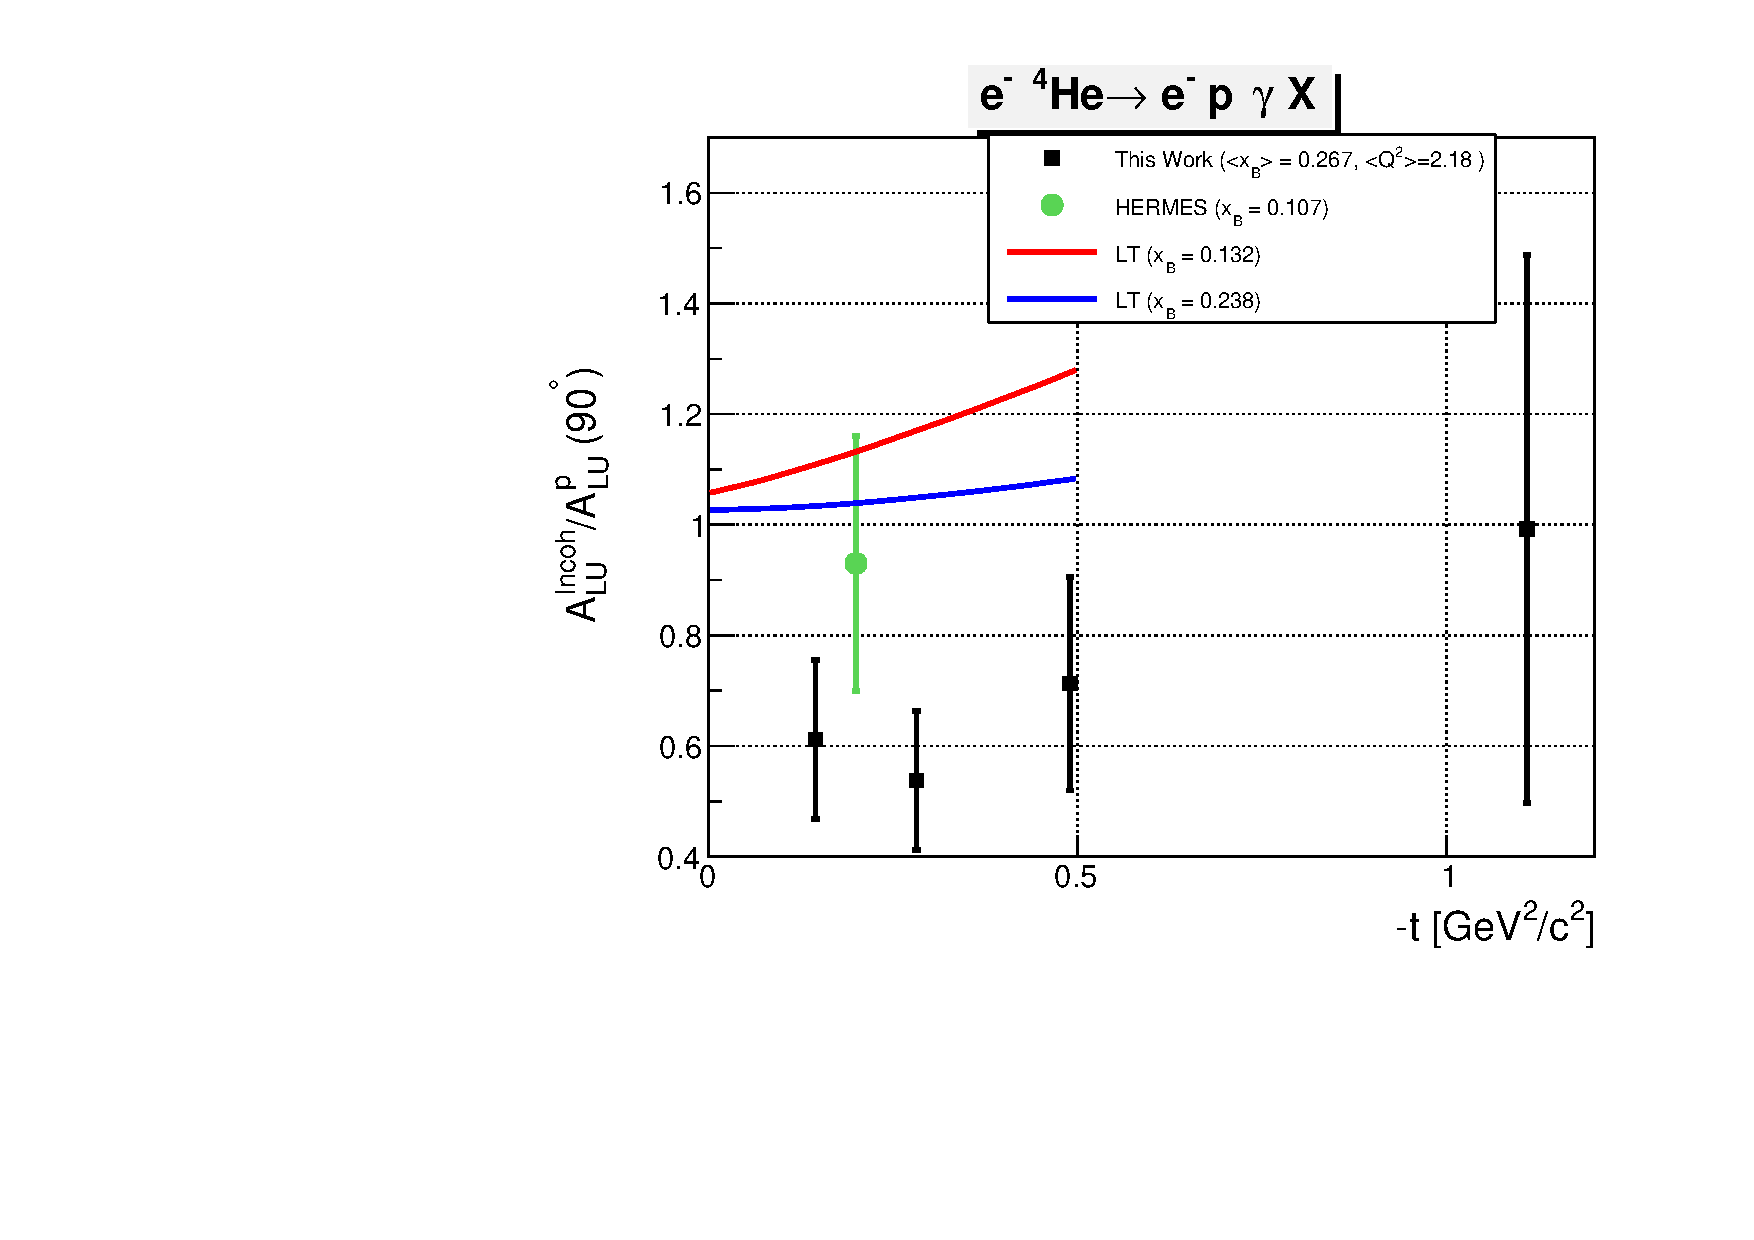
\includegraphics[height=6.6cm]{fig/BSA_ratio_incoh_t.pdf}
    \caption{ $A_{LU}$ ratio between bound proton and free proton at $\phi =  
    90 ^{\circ}$ as a function of $Q^{2}$, $x_{B}$, and $-t$.}
    \label{fig:incoh-alu-ratios}
    \end{figure}





\item CFF: the committee acknowledges that the new procedure (2-parameter fit 
with complete formula at leading-twist) is more satisfying. It recommends 
though to be cautious about the statements on CFF in the future publication.

\item CAN: a number of answers to previous questions have to appear in the CAN.  
This includes (but may not be limited to) 

Figs 1-4 of \url{https://clasweb.jlab.org/rungroups/lowq/wiki/images/a/a3/Final_1st_round_comments.pdf} 
Tighter $edist$ cut [-2,+3 mm].
Otherwise, even if you do not show it in the CAN, mention in one line that a 
specific study was done.
\item Miscellaneous:
   \begin{enumerate}
      \item 4-D dependences of the ratio R: the statement that the integrated R's 
    are flat is disputable (see Figs 4.16 and 4.17), but we are ready to accept 
    that the effect discussed is small and taken care of in the systematic 
    errors.\\
    \textcolor{blue}{We implemented a 4D ratio R for the background 
       subtraction. The difference between the reconstructed ALU with 2D and 4D 
       background subtraction are presented in figures \ref{fig:coh_binning} 
       and \ref{fig:incoh_binning} for the coherent and the incoherent DVCS 
       channels. Even though the 2D was a good a pproximation, a 4D subtraction 
    is applied on the final results.} 
    \begin{figure}[tbp]
    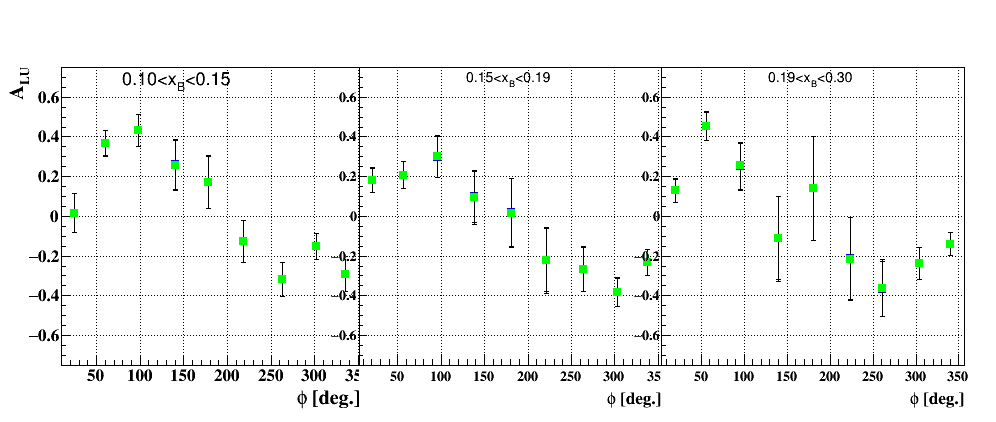
\includegraphics[height=6.6cm]{fig/BSA_Coherent_xB.png}
    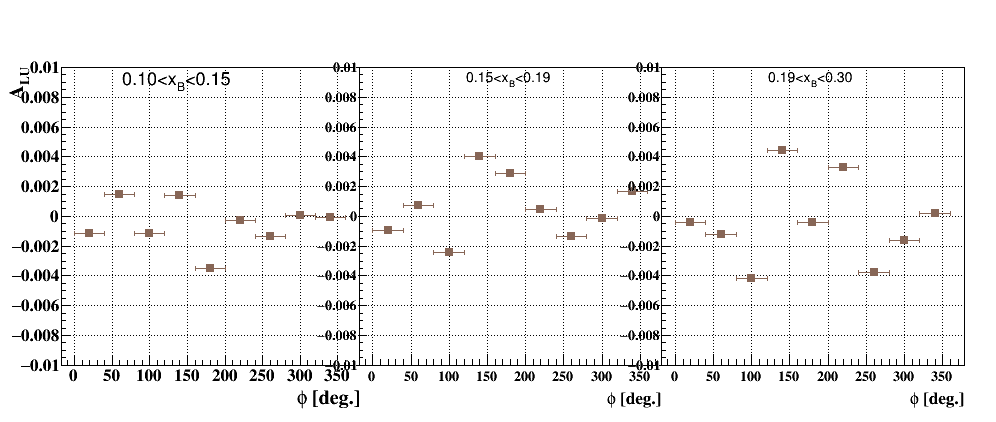
\includegraphics[height=6.6cm]{fig/diff_BSA_Coherent_xB.png}
    \caption{On top: the reconstruct coherent beam-spin asymmetries as a 
    function of $\phi$ in $x_{B}$ bins using 2D (in blue) and 4D (in green) 
 background subtraction.  On bottom: the difference between the two asymmetries 
 as a function of $\phi$.}
    \label{fig:coh_binning}
    \end{figure}            

    \begin{figure}[tbp]
    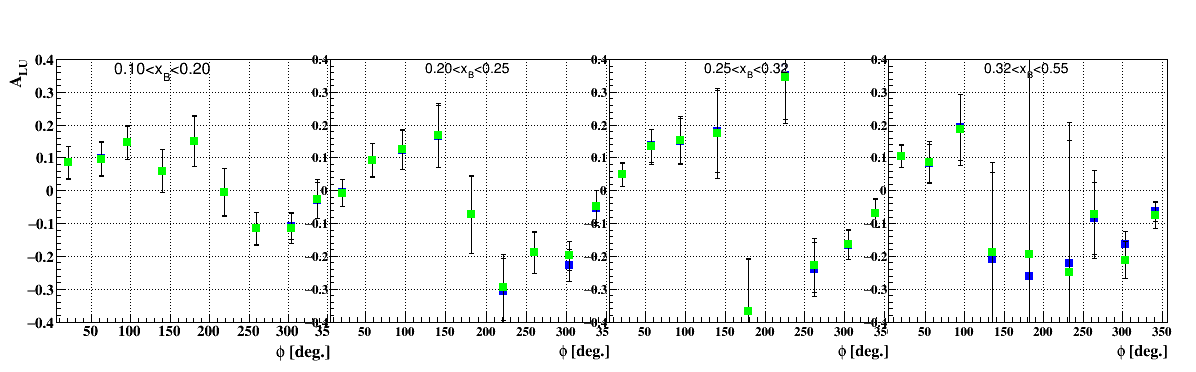
\includegraphics[height=5.6cm]{fig/BSA_InCoherent_xB.png}
    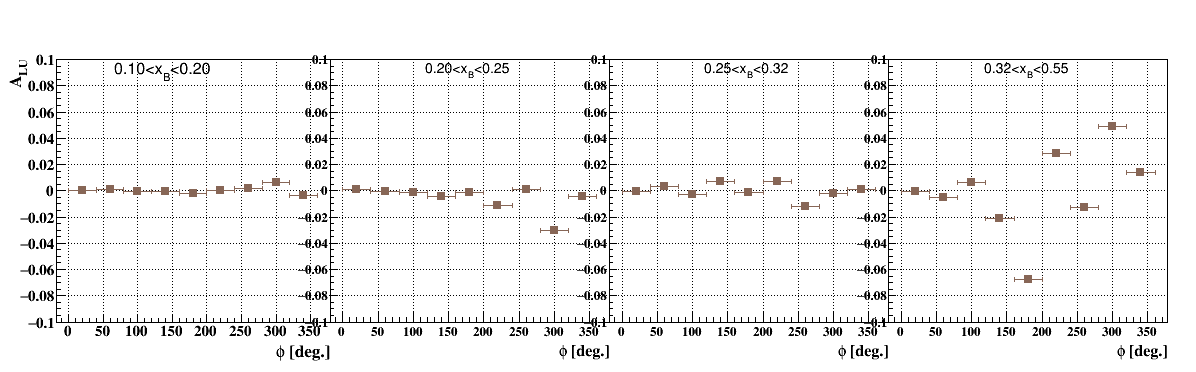
\includegraphics[height=5.6cm]{fig/diff_BSA_InCoherent_xB.png}
    \caption{On top: the reconstruct incoherent beam-spin asymmetries using 2D   
    (in blue) and 4D (in green) background subtraction. On bottom: the 
 difference between the two asymmetries as a function of $\phi$.}
    \label{fig:incoh_binning}
    \end{figure}                                                                  



 \item not convinced that comparing 9 phi-bins to 11 is a definitive answer, 
    when not applying any finite bin size correction. But again, in view of the 
    size of statistical and systematic errors, would accept that.

\item Your Eq.(4) of "answer" is probably wrong. For our own understanding, 
   look into this argument again.

   \end{enumerate}

\item Please keep a record of the changes in the CAN, as we will probably not 
re-read the whole text.

\item Request to see the very first draft of the publication.

\end{enumerate}
